\renewcommand{\thechapter}{\arabic{chapter}}
\setcounter{chapter}{2}

\chapter{Intelligence artificielle et notions complémentaires}
\label{chap:chapter_3}
\chapterintro
Lors du précédent chapitre, les interactions entre la peau et la lumière ont été abordées, ainsi que les dispositifs majeurs permettant l'acquisition d'informations de la peau.\par

Actuellement, l’informatique est une ressource omniprésente dans de nombreux domaines d’application. Ses facultés à divertir ou encore à guider ses usagers dans leurs choix quotidiens personnels et professionnels en font un précieux allié. De nouvelles pratiques font leurs apparitions, intégrant la machine au cœur des processus décisionnels. Les disciplines médicales évoluent largement et l’ordinateur permet de répondre aux besoins croissants de précision, de reproductibilité intra et inter opérateur, et permet un gain de temps au sein des milieux cliniques. Dans un cadre bien défini, il s’agit également d’un moyen de formaliser la connaissance au travers d’un outil pouvant être utilisé par des non-initiés.\par

Cette nouvelle partie permet de dérouler un peu plus le plan de ce manuscrit, en abordant cette fois-ci les systèmes d'intelligence artificielle et leur utilité vis-à-vis des données médicales à la disposition de ce travail.\par
\newpage

\section{Généralités sur l'intelligence artificielle}
\label{sec:artificial_intelligence}
La notion \textbf{d’\gls{ia}} est assez souvent contestée, mais se définit plus généralement comme étant «~l’ensemble de théories et de techniques mises en œuvre en vue de réaliser des machines capables de simuler l'intelligence humaine~»~\textsuperscript{\ref{footnote:ia_larousse}}. Ainsi, dans cette définition, ces techniques ne se limitent pas à la reproduction du comportement interactif social humain souvent représenté dans les médias. La mise en pratique sous forme informatique de mécanismes dédiés à la prise de décision à partir de données ou encore, la retranscription du raisonnement d'un expert fait partie de cette définition.\par

Une vision plus complète de ce terme consiste à décomposer l'\gls{ia} en une discipline organisée en sous domaines possédant chacun leurs spécificités, comme schématisé sur la \Cref{fig:scheme_overview_ia}. Ainsi, le terme \textbf{d'apprentissage automatique} ou de \textit{machine learning} caractérise un premier sous champ de l'\gls{ia} et est employé pour qualifier l'utilisation de mécanismes statistiques dans le but de générer des règles, à partir de données d'apprentissage. Ces données étant souvent complexes, il est souvent nécessaire de laisser l'humain intervenir pour extraire l'information pertinente à l'accomplissement de la tâche souhaitée. Enfin, le terme \textbf{d'apprentissage profond} ou de \textit{Deep Learning} désigne un sous champ de l'apprentissage automatique, dans lequel des couches succesives de prises de décision vont permettre d'augmenter la complexité des relations entre les données d'entrée et les tâches.\par

\addtocounter{footnote}{1}
\footnotetext[\thefootnote]{Source~:~Encyclopédie Larousse. \label{footnote:ia_larousse}}

\begin{figure}[H]
    \centering
    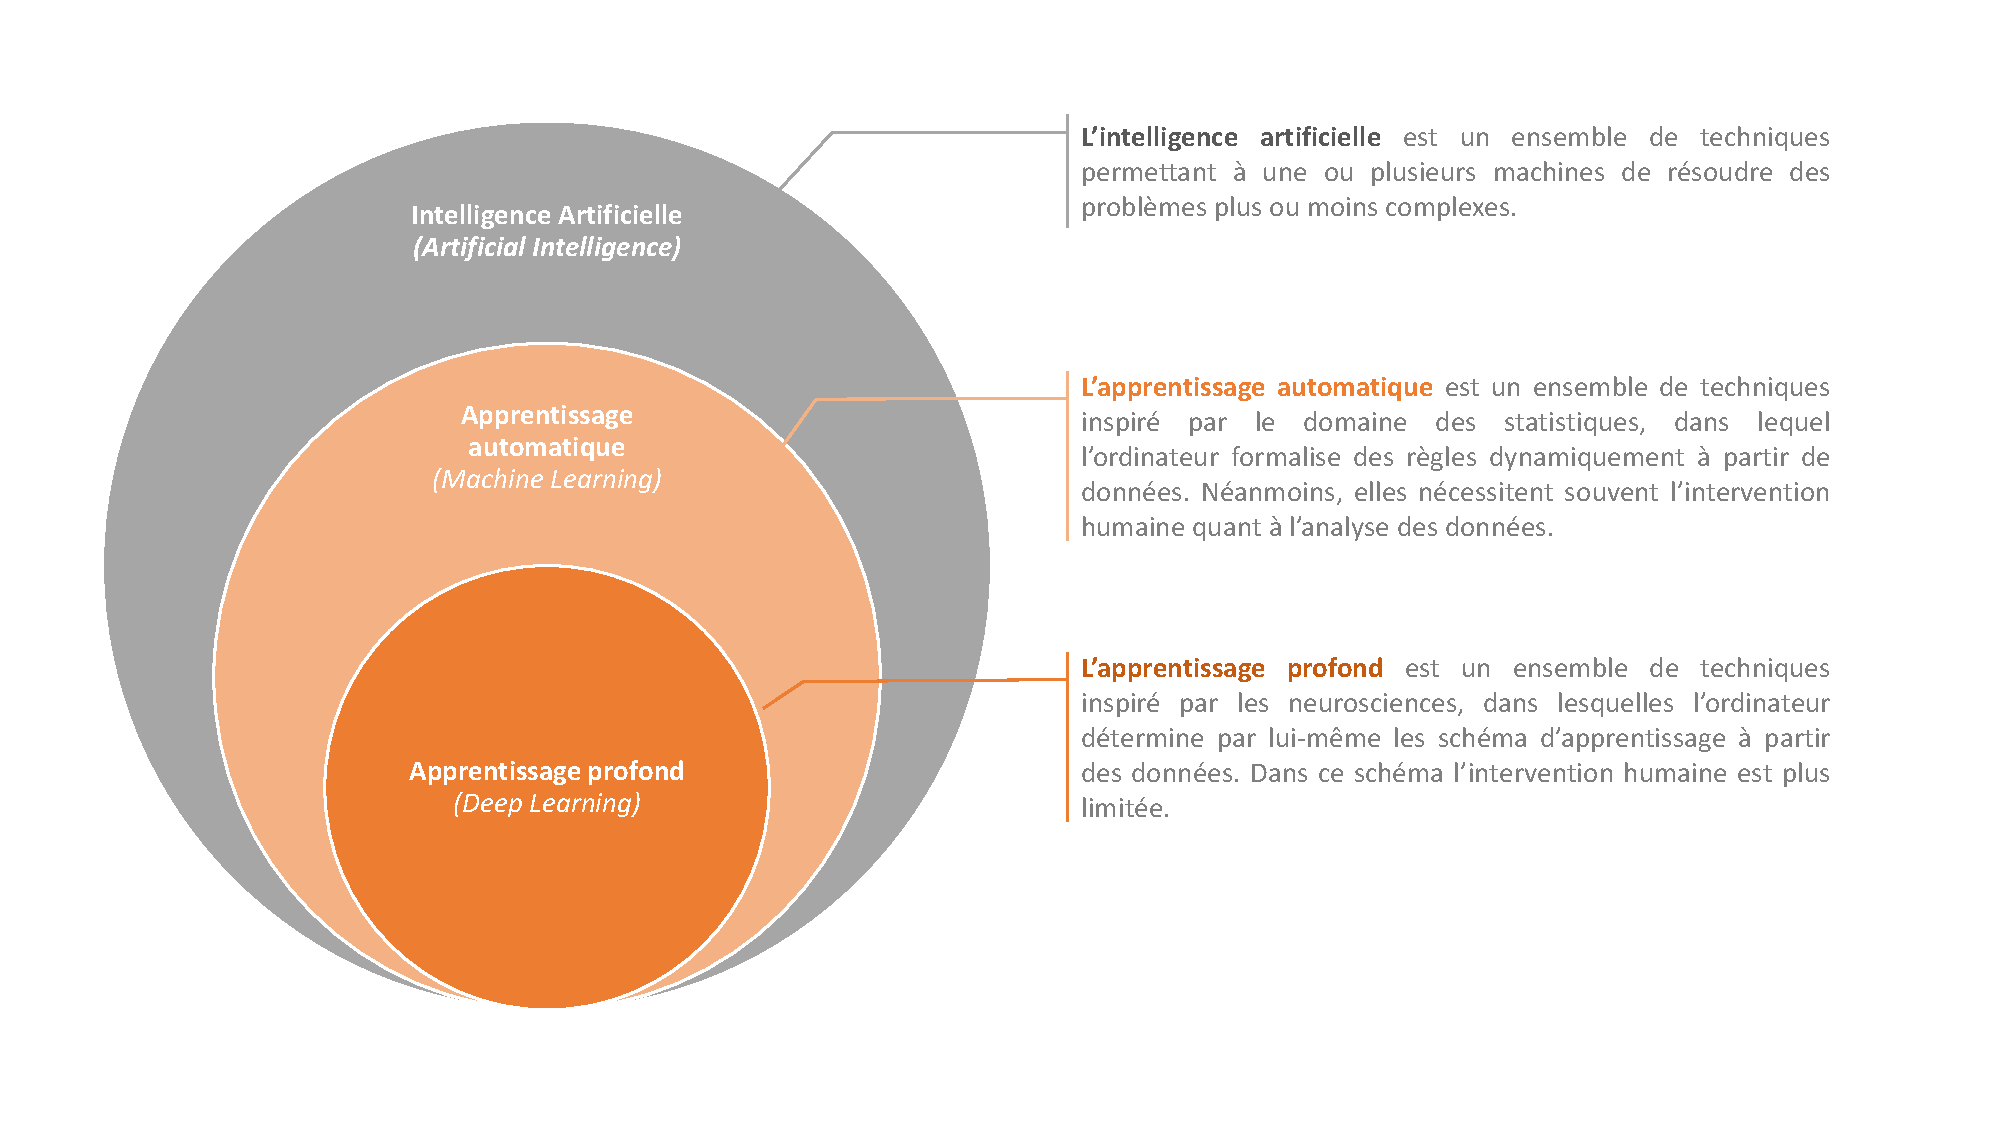
\includegraphics[width=\linewidth]{contents/chapter_3/resources/scheme_overview_ia.pdf}
    \caption{Représentation des relations entre \textit{intelligence artificielle}, \textit{apprentissage automatique} et \textit{apprentissage profond}.}
    \label{fig:scheme_overview_ia}
\end{figure}\par

Cette partie a pour vocation d’amener à la compréhension générale des courants d’\gls{ia}, qui permettent la résolution de problématiques variées telles que la dermatologie. Dans une première section, les approches par apprentissage sont décrites, puis par extension amène à la présentation de l'apprentissage profond dans une seconde section. La troisième section décrit les méthodes permettant le paramétrage et l'évaluation de ces modèles. Enfin, la dernière section décrit les principes de fusions utiles à ce travail.\par

\section{Approches par apprentissage}
\label{sec:machine_learning}
Ce courant a été \textit{évoqué} en 1948 par Alan Turing ; son idée était de proposer des «~machines à apprendre susceptibles de construire elles-mêmes leurs propres codes~»~\cite{Turing1950}. En 1959, Arthur Samuel formule une première définition des approches par apprentissage comme étant un « domaine d’étude dans lequel la possibilité est donnée à l’ordinateur d’apprendre sans avoir été explicitement programmé ».\par 

Les approches par apprentissage automatique peuvent être résumées aux techniques permettant à un système informatique d’adapter son analyse et son comportement en fonction de ses données d’entrée. Une définition plus formelle et récente de ce domaine proposée par Tom Michael Mitchell est qu’un «~programme informatique apprend d’une expérience $E$, en adéquation avec des tâches $T$ et une mesure de performance $P$, si sa performance sur les tâches $T$, mesurée par $P$, s’améliore avec l’expérience $E$~».\par

Ainsi au sein des courants d’apprentissage, deux grandes sous catégories synthétisées dans la \Cref{fig:scheme_machine_learning} peuvent être distinguées, dont~:~
\begin{itemize}
    \item l'apprentissage \textbf{supervisé} correspond aux techniques visant à faire correspondre les données d'entrée avec des sorties de valeurs discrètes (on parle aussi de classification) ou continues (on parle alors de régression),
    \item l'apprentissage \textbf{non-supervisé} correspond à des approches exploratoires, dans lesquelles l'ordinateur tente d'identifier des corrélations au sein des données (désigné par le terme de \textit{clustering}),
    \item l'apprentissage \textbf{semi-supervisé}~\cite{Robert2014} reprend les précédentes théories afin d'exploiter au mieux l'ensemble des données à disposition et de mieux discerner le problème.
\end{itemize}

Les prochaines sous-sections de ce chapitre abordent chacune de ces catégories respectives de manière plus détaillée.\par
 
\begin{figure}[H]
    \centering 
    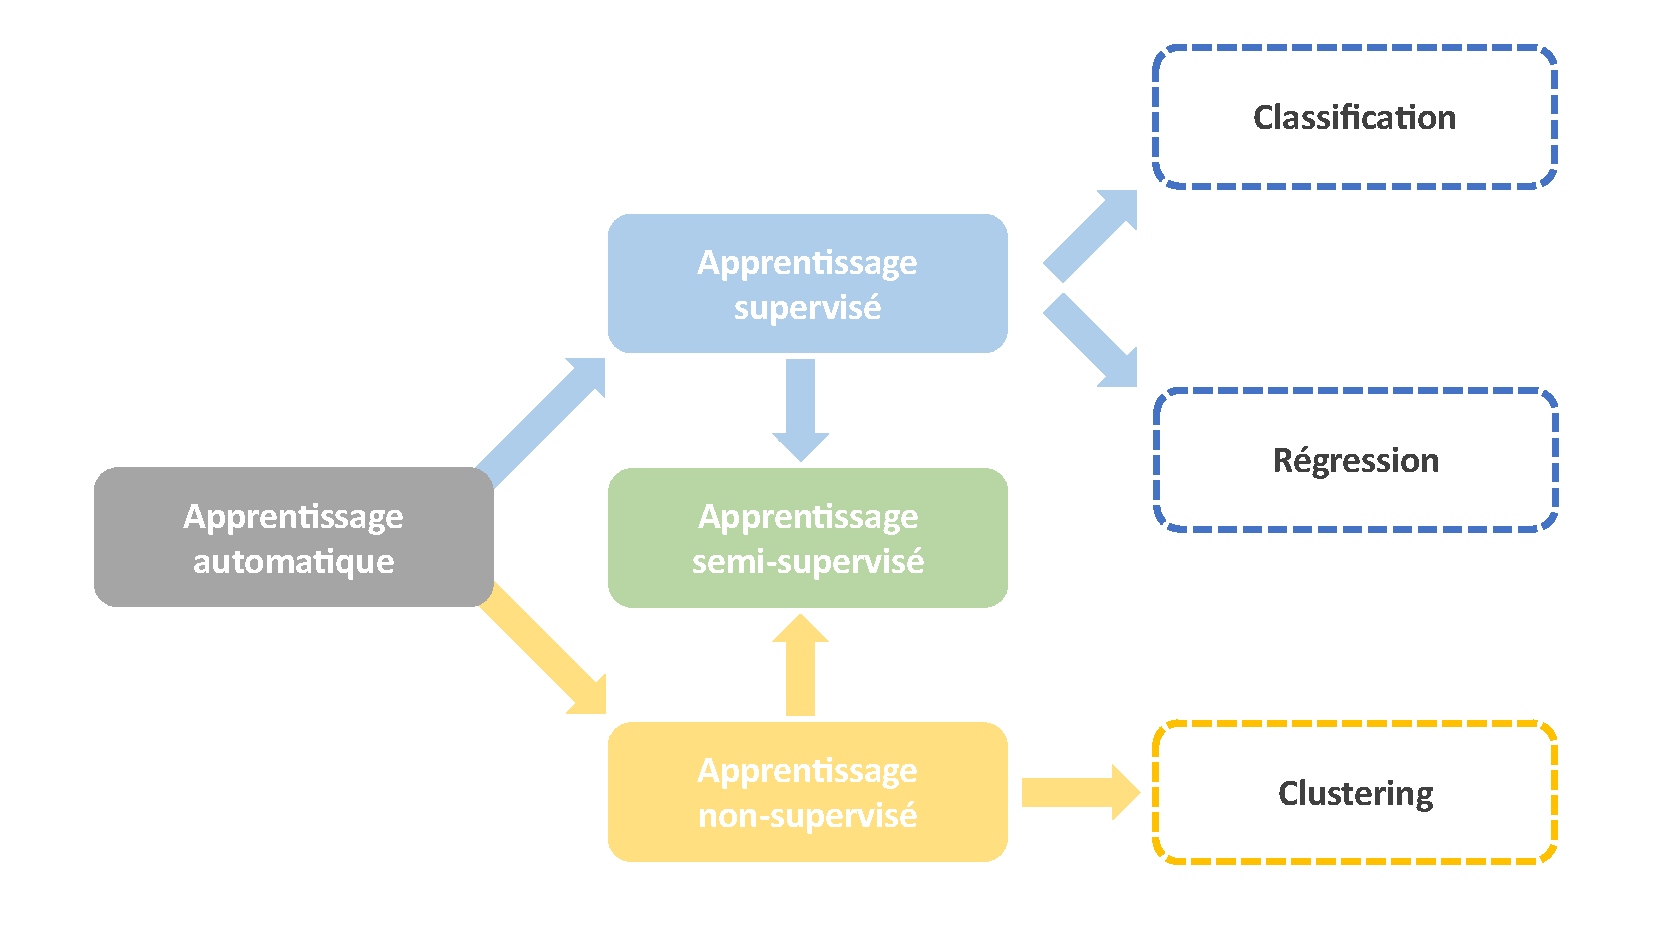
\includegraphics[width=\linewidth]{contents/chapter_3/resources/scheme_machine_learning.pdf}
    \caption{Schéma de décomposition des approches par apprentissage automatique.}
    \label{fig:scheme_machine_learning}
\end{figure}

\subsection{Apprentissage supervisé}
\label{sec:supervised_learning}
L’apprentissage supervisé consiste à déterminer la relation permettant de faire correspondre des données d’entrée $x$ et des données de sorties $y$ et cela, dans le but de produire sur de nouvelles données d’entrée $x'$, de nouvelles sorties $y'$.\par

Cette approche implique l’utilisation d’une base d’apprentissage, définie comme \textit{un ensemble de couples entrée-sortie} noté $\{(x_1,y_1 ),\ldots,(x_n,y_n )\}$ avec $n \in N$. Ainsi, l’humain tente d'apporter une signification à ces données sous forme d'annotations (ou étiquettes) pour lesquelles la machine devra être en mesure de déterminer la relation existante.\par

Dans le but d'achever cette tâche, les variables propres à chaque observation sont supposées suffisamment discriminantes pour permettre l'identification des annotations. Ce problème est défini par la relation $y=f(x)$, où $f$ est une fonction inconnue correspondant au phénomène observé, par une fonction d’approche $g$ appelée fonction de prédiction tel que $y=g(x)$, avec $x=\{x_1,x_2,\ldots,x_n\}$ un vecteur de caractéristiques possédant suffisamment d'information~\cite{foulds2010}.\par 

Cet apprentissage, schématisé sur la \Cref{fig:scheme_supervised_classification}, se découpe en deux processus distincts~:
\begin{itemize}
    \item \textbf{l’apprentissage} ou \textit{entraînement}, qui consiste à approcher la fonction $f$ par une fonction $g$ compte tenue de données étiquetées,
    \item \textbf{la prédiction} ou \textit{inférence}, qui consiste à prédire sur de nouvelles données à partir de $g$ tel que $g(x') = y'$.
\end{itemize}\par

\begin{figure}[H]
    \centering
    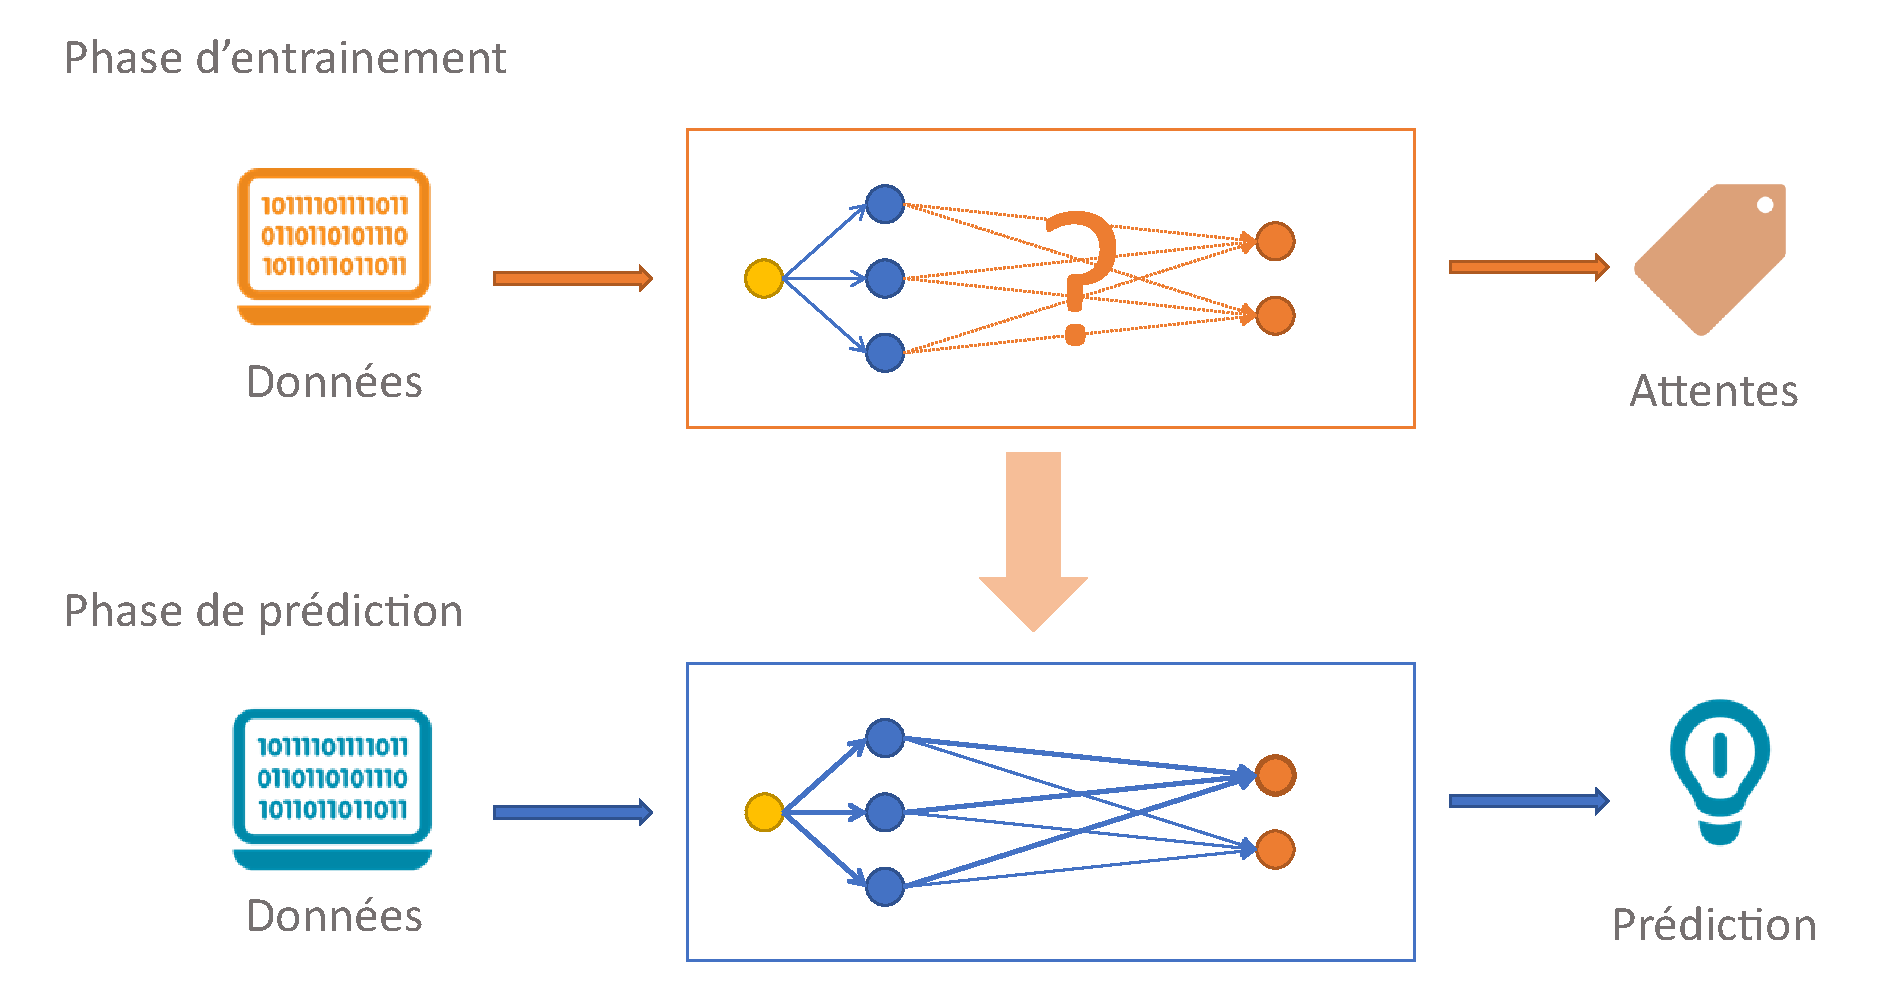
\includegraphics[width=\linewidth]{contents/chapter_3/resources/scheme_supervised_classification.pdf}
    \caption{Schéma de l’approche dite supervisée. La phase d'entraînement permet de déterminer les relations entre données et attentes, sur des données connues dites d'apprentissage. La phase de prédiction réutilise les relation déterminées lors de la phase d'entraînement. }
    \label{fig:scheme_supervised_classification}
\end{figure}
\clearpage

Ces approches dites supervisées se regroupent ainsi au travers de deux catégories majeures~:
\begin{itemize}
    \item la \textbf{classification}, c’est-à-dire la prédiction de valeurs discrètes, soit l’ensemble des entiers relatifs noté $\pmb{\mathbb{Z}}$. Sont également utilisés les compléments de \textit{classification binaire} lorsque le problème formulé ne comporte que deux classes, et de \textit{classification multi-classes} lorsque la situation nécessite de prédire $N$ classes avec $N > 2$.
    \item la \textbf{régression}, c’est-à-dire la prédiction de valeurs continues, soit l’ensemble des nombres réels noté $\pmb{\mathbb{R}}$.
\end{itemize}\par

Les travaux de ce manuscrit portent sur les méthodes de classification, qui se traduisent par la catégorisation d'images cliniques pathologiques ou de lésions selon divers niveaux de dangerosité. En prenant appui sur l'un des travaux~\cite{Kotsiantis2007}, une synthèse de ces méthodes et de leur principe respectif est fournie, dont~:
\begin{itemize}
    \item \textbf{les approches logiques} qui correspondent à des approches par succession de décisions~\cite{Kotsiantis2007}. Dans cette catégorie, le principal représentant est celui des arbres de décision~\cite{Breiman1984}, également connu sous le terme de \gls{cart}, dont le principe peut se résumer à la construction d'un graphe, dans lequel chaque noeud est associé à une décision définie par le choix d'une caractéristique et d'un seuil~\cite{Quinlan1986}. Toute la complexité de ces approches repose sur le choix de ces caractéristiques dont la priorité dépend de l'ordre d'importance dans la séparation du problème.
    \item \textbf{les approches statistiques} qui correspondent à des approches probabilistes, qui déterminent la probabilité d'appartenance d'un élément à une classe. Le \gls{nbm}~\cite{Zhang2004} est un exemple typique de ce type d'approche, dans lequel chaque caractéristique est considérée comme indépendante. La relation entre caractéristique et annotation se définit ainsi comme le produit des probabilités de chacune d'entre elles d'appartenir à la classe supposée (voir l'\Cref{eq:bayesian}). Ce type de classification bayésienne peut également être étendue sous la forme de réseau~\cite{Kononenko1989}.
    \item \textbf{les approches par instances} qui qualifient des méthodes consistant à une accumulation des échantillons afin d'enrichir un espace et non pas de leur interprétation menant à une forme de connaissances. La méthode la plus connue reposant sur ce principe est celle des \gls{knn}~\cite{Cover1967}, dont la théorie majeure repose sur l'appartenance d'une donnée à une classe si celle-ci est suffisamment proche par ses caractéristiques, d'échantillons pré-existants de cette dernière. Il est alors nécessaire de définir un critère de distance, le principal utilisé étant celui de la distance euclidienne. 
    \item \textbf{les approches par \gls{svm}}~\cite{Cortes1995} correspondent à des approches assez récentes dont le principe se résume à déterminer une frontière de séparation entre les diverses classes, qui maximise une marge suffisante permettant entre autres une meilleure tolérance au bruit. Afin de déterminer au mieux cette frontière, divers noyaux ont été établis dont le plus simple d'entre eux est \textbf{le noyau linéaire}. La présence \textbf{d'un noyau de fonction de base radiale} ou \textit{Radial Basis Function} est à préciser, considéré comme un \textit{approximateur universel} si les données à disposition sont suffisantes~\cite{Wang2004}.
    \item \textbf{les approches par ensembles} sont une catégorie qui qualifie les méthodes qui emploient un ensemble de modèles prédictifs afin de construire un unique modèle plus robuste. L'une de ces méthodes, les \gls{rf}~\cite{Breiman2001} sont une extension du principe d'arbre de décision précédemment évoqué, destiné à réduire le risque de sur-apprentissage du modèle initial. Cette méthode réalise $N$ sélections aléatoires d'observations, pour lequel $N$ arbres de décision sont générés. Afin de diversifier ces arbres, un mécanisme de tirages aléatoires de caractéristiques est également réalisé au niveau de chaque noeud de décision. Une autre de ces méthodes, l'\gls{gb} est un mode opératoire généralement constitué par des arbres de décisions. En opposition avec les \gls{rf} où chaque arbre de décision correspond à un modèle de prédiction faible, l'\gls{gb} consiste à diminuer de manière séquentielle une fonction de coût à chaque nouvel arbre généré~\cite{Friedman2001}.
\end{itemize}\par

\begin{equation} 
    \label{eq:bayesian}
    \hat{y} = \underset{k \in \{1, \ldots, K\}}{\operatorname{argmax}} \ p(C_k) \displaystyle\prod_{i=1}^n p(x_i \mid C_k)
\end{equation}

Devant ces nombreuses méthodes, il est difficile de déterminer un modèle optimal à une situation particulière, notamment dans le cadre de données à forte complexité. En effet, une évaluation de manière empirique de ces diverses méthodes reste encore la meilleure solution afin de déterminer ce modèle optimal, en contrepartie d'un temps de calcul important. Néanmoins, l'un des travaux menés sur la performance des modèles supervisés, a permis de déterminer un certain nombre de critères de comparaison entre ces diverses techniques mettant en valeur en général les avantages et inconvénients de chacune d'entre elles~\cite{Kotsiantis2007}.\par

Pour cela, la \Cref{tab:model_comparison} recense la plupart des critères importants évoqués par ce travail de recherche. La performance de classification notamment, qui semble indéniable dans le champ que ce travail tente d'évaluer avec une emphase forte en termes de performances pour les \gls{svm}. La vitesse d'apprentissage a également été précisée à titre indicatif. En effet, bien que contraignante lors des expérimentations de ce manuscrit, elle ne constitue pas un frein et reste le principal inconvénient des \gls{svm}. Enfin, ces derniers sont reconnus comme robustes face à des situations pouvant comporter des caractéristiques non pertinentes ou redondantes.\par

À la vue de ces éléments, il semble plus que nécessaire de considérer l'utilisation des \gls{svm} au sein de ces travaux. De même, il est nécessaire de considérer l'utilisation des deux méthodes d'approches par ensemble mentionnées, les \gls{rf} et l'\gls{gb}, pour lesquelles aucun travail comparatif généraliste n'a été trouvé. Néanmoins, une étude génomique semble plaider dans le sens des \gls{svm} et de l'\gls{gb}~\cite{Ogutu2011}. Pour finir, il est également nécessaire de considérer ces modèles de classification au sein de processus proposés par des travaux proches de cette thématique. Ces éléments sont abordés plus en détail dans leur partie respective.\par

\begin{table}[H]
  \small
  \centering 
    \begin{tabular}{lcccc}
        \toprule
                                                                    & \textbf{\gls{cart}}   & \textbf{\gls{nbm}}& \textbf{\gls{knn}}    & \textbf{\gls{svm}}\\
        \midrule
        \textbf{Performances de classification}                     & **                    & *                 & **                    & ****              \\
        \midrule
        \textbf{Vitesse d'apprentissage}                            & ***                   & ****              & ****                  & *                 \\
        \midrule
        \textbf{Tolérance aux caractéristiques non pertinentes}     & ***                   & **                & **                    & ****              \\
        \midrule
        \textbf{Tolérance aux caractéristiques redondantes}         & **                    & **                & **                    & ***               \\
        \bottomrule
  \end{tabular}
  \caption{Table de comparaison des méthodes d'apprentissage majeures de la littérature~\cite{Kotsiantis2007}. Ce tableau propose un système de notations allant de une (mauvaise performance) à quatre étoiles (bonne performance).}
  \label{tab:model_comparison}
\end{table}
\clearpage

\subsection{Apprentissage non-supervisé}
\label{sec:unsupervised_learning}
L’apprentissage non supervisé ou \textit{descriptif} est une seconde approche d’apprentissage dans laquelle l’ordinateur tente de \textit{découvrir} en autonomie, des corrélations au sein de jeux de données. Ces approches émergent de problématiques diverses, telles que~:
\begin{itemize}
    \item la \textbf{réduction des coûts} le plus souvent humain nécessaire à l’obtention de données annotées, c’est-à-dire de données pour lesquelles les couples d’entrées et de sorties sont connus.
    \item la \textbf{découverte des diverses relations} pouvant exister au sein d’un amas de données. En effet, une annotation ne correspond qu'à un échantillon de l’information et ne permet pas d’obtenir les relations pouvant régir des modèles d'interactions complexes.
    \item l'\textbf{exploration de nouvelles relations} de type \textit{cause – effet}, en réaction à la masse de données produites par les objets connectés.
\end{itemize}\par

Ce principe est concrétisé aux travers de méthodes, comme les k-moyennes qui tentent de déterminer des correspondances en minimisant la différence d’énergie entre les points d’un même groupe, dont un schéma est visible sur la \Cref{fig:scheme_unsupervised}. Diverses applications peuvent ainsi en résulter, telles que~:
\begin{itemize}
	\item le \textbf{regroupement par classes de données}, afin de définir de manière automatique de nouvelles annotations.
	\item la \textbf{réduction de dimensions}, dans le but de ne conserver que l'information essentielle. La méthode du \textit{bag-of-words} est un exemple initialement prévue pour l'analyse de texte~\cite{Zhang2010} et utilisée dans des domaines tels que l'analyse d'image de la peau~\cite{Situ2008}.
	\item la \textbf{découverte de relations} au sein de l’information, et des relations les plus robustes entre variables et dépendances.
\end{itemize}\par

\begin{figure}[H]
    \centering
    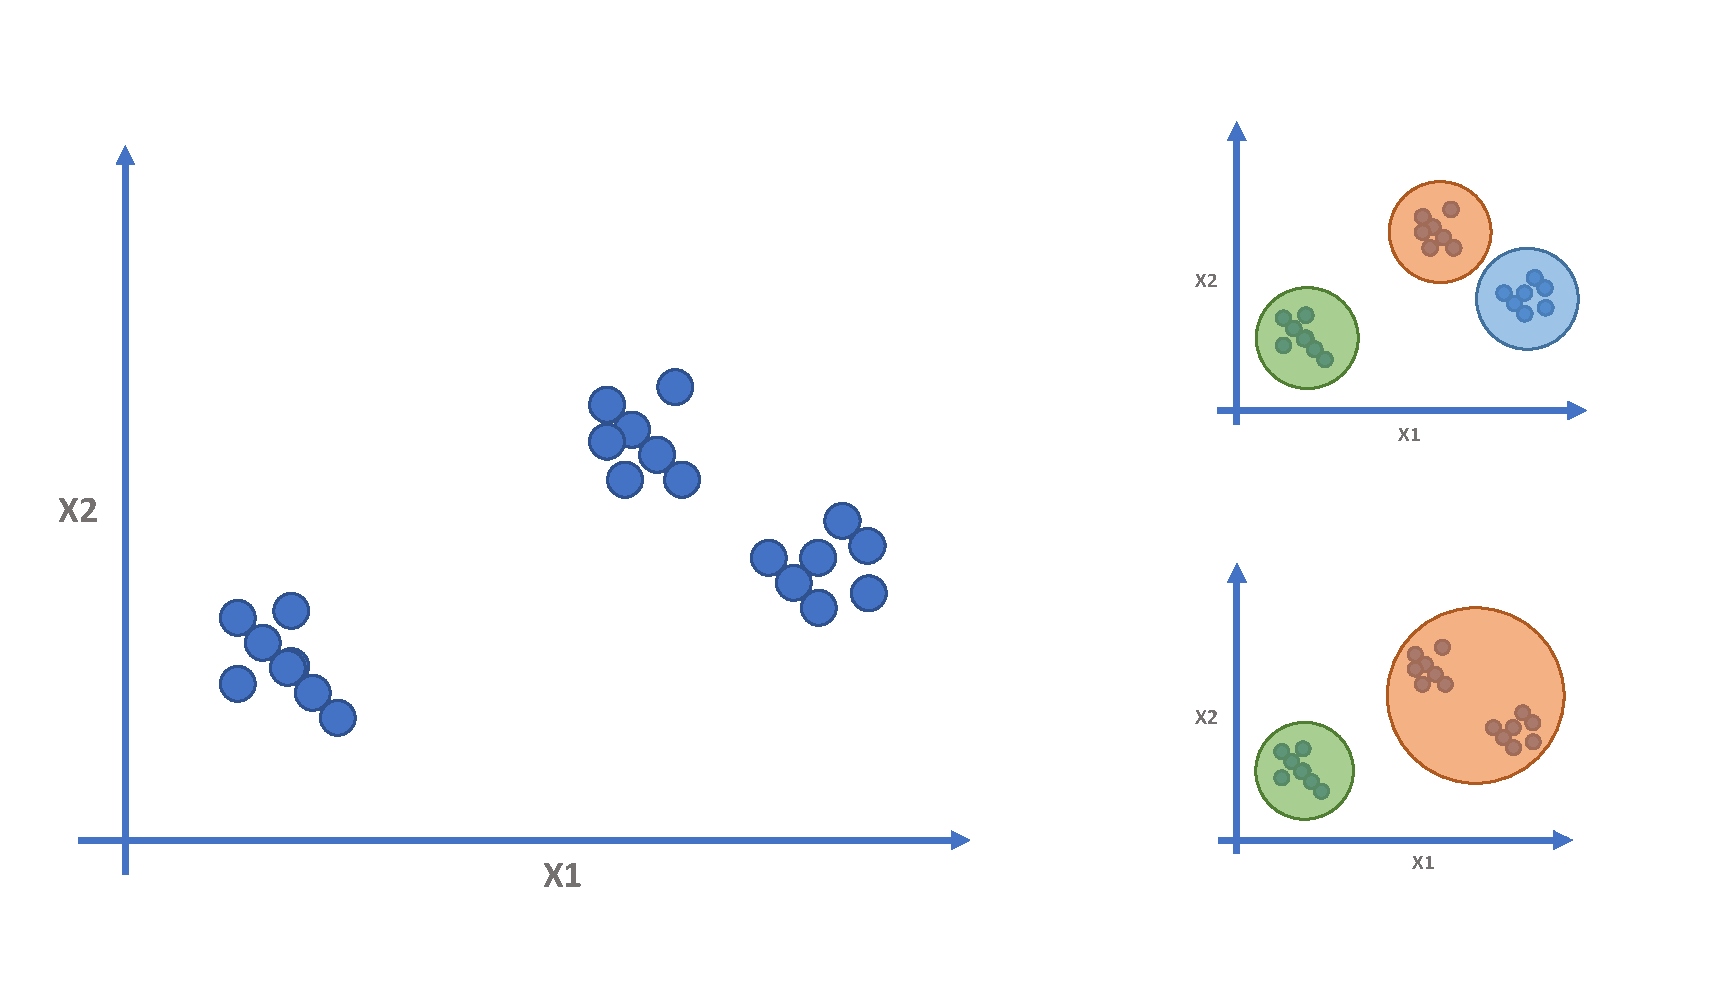
\includegraphics[width=0.9\linewidth]{contents/chapter_3/resources/scheme_unsupervised.pdf}
    \caption{Exemple de données non associées à des annotations préalables, et pour lesquelles des approches non supervisées peuvent être sollicitées afin de découvrir des groupes de données ou \textit{clusters}. Le nombre de groupes le plus souvent défini par l’utilisateur avant traitement, influe fortement la vision du problème.}
    \label{fig:scheme_unsupervised}
\end{figure}

\subsection{Apprentissage semi-supervisé}
\label{sec:semisupervised_learning}
Les techniques d'apprentissage semi-supervisé tentent de combiner les deux principes précédents et sont la conséquence du coût de l'annotation des données qui nécessite souvent le travail d'experts. En effet, il peut être difficile d'avoir accès à une vérité terrain qui couvre la totalité d'un jeu de données sans pour autant perdre l'apport de cette information non-annotée. Ce dernier point est particulièrement intéressant dans le cadre de données à grande dimensions pour lesquelles \textbf{l'espace} des dimensions croît de manière exponentielle et \textit{dilue} les échantillons (connu sous le terme de \textit{fléau des dimensions}~\cite{Donoho2000}).\par 

Ainsi, l'apprentissage semi-supervisé se base sur plusieurs hypothèses auxquelles doivent se confronter les données~\cite{Zhu2009}, dont~:
\begin{itemize}
	\item un critère \textbf{d'homogénéité}, c’est-à-dire que des données issues d'une zone de haute densité partagent les mêmes annotations, 
	\item un critère \textbf{de séparation par faible densité}, c’est-à-dire que s'il existe une  séparation entre plusieurs types d'annotations, celle-ci se situant dans une zone à faible densité~\cite{chapelle2005}.
\end{itemize}
En pratique, il est difficile de s'assurer que des données mises à disposition respectent bien ces engagements. Afin de mieux visualiser ce concept, l'exemple en \Cref{fig:example_semi_supervised} démontre l'intérêt de telles approches. Ce principe permet d'éviter d'extrapoler des frontières difficilement définissables dans une situation de faible densité de l'information étiquetée.\par
 
\begin{figure}[H]
    \centering
    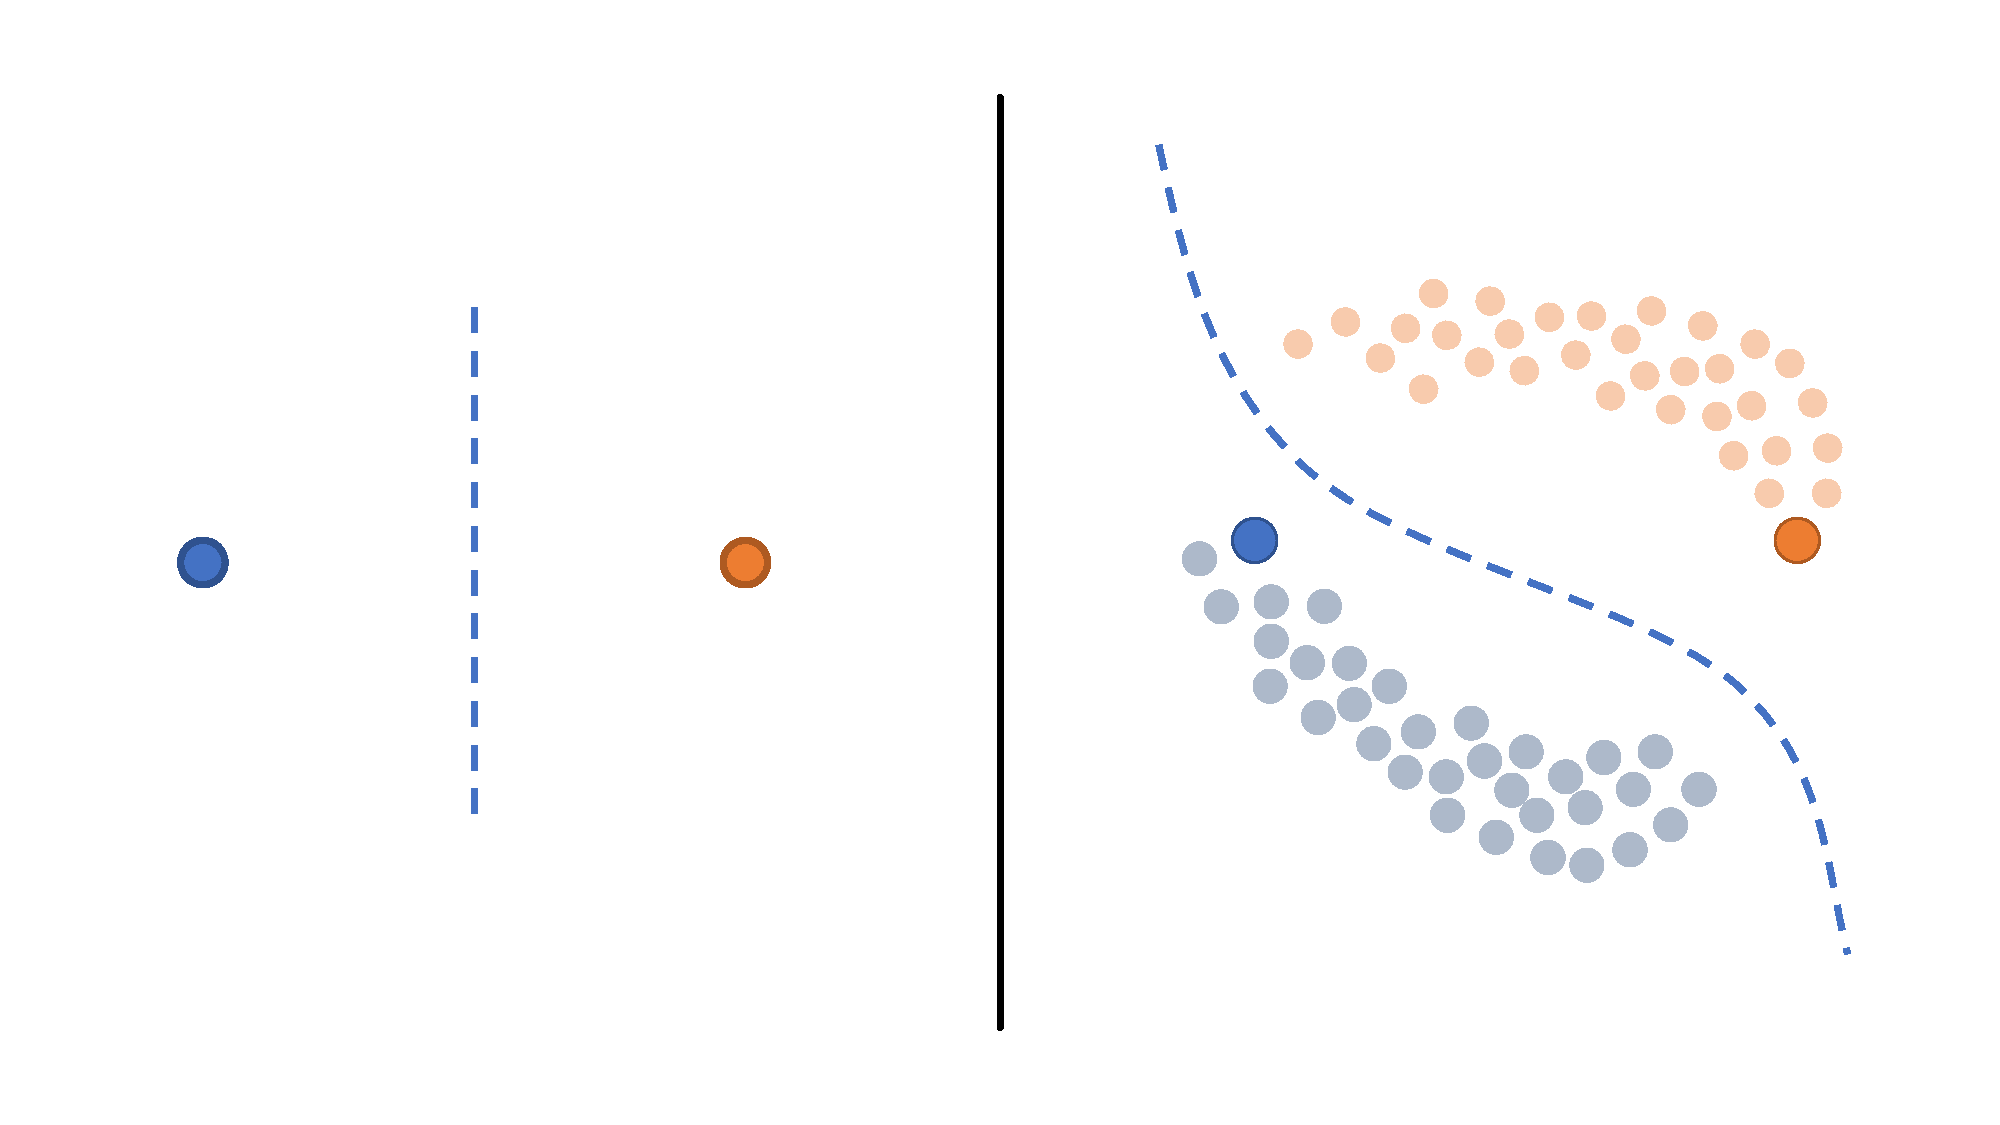
\includegraphics[width=\linewidth]{contents/chapter_3/resources/example_semi_supervised.pdf}
    \caption{Exemple fréquemment employé pour démontrer l'intérêt de l'apprentissage semi-supervisé du point de vue du principe de densité. À gauche, une classification obtenue à partir de deux données étiquetées ; À droite, la même situation avec l’ajout de données non étiquetées.}
    \label{fig:example_semi_supervised}
\end{figure}

\clearpage

\section{Apprentissage profond}
\label{sec:deep_learning}
L’apprentissage profond correspond à un sous-ensemble de l’apprentissage automatique, encouragé par les récents apports des neurosciences sur le fonctionnement et le rôle des neurones sur la prise de décisions complexes~\cite{Quartz1997,Shrager1996}. En effet, le cerveau possède divers niveaux de traitement de l’information, ce que tente d'imiter l'apprentissage profond par l'apport de multiples couches de traitement.\par

En effet, dans le cadre des méthodes \textit{classiques} d’apprentissage évoquées dans la partie précédente, la dimension de \textit{couches} de traitement n’est pas intégrée. Les approches par apprentissage simple proposent une architecture en trois couches, dont l’une des couches est allouée à la corrélation entre les données d’entrée et de sortie. Par opposition, les approches par apprentissage profond proposant des structures en $n$ couches, avec $n \in \pmb{\mathbb{N}}$ et $n>1$. Ces couches intermédiaires sont également qualifiées de couches cachées.\par 

Dans une première sous-section, une brève présentation du principe de \gls{ann} est réalisé, puis dans une seconde sous-section est détaillée leur extension au \gls{cnn}. Enfin, les aspects liés au principe de transfert de connaissances sont proposés dans une dernière sous-section.\par

\subsection{Réseau de neurones artificiels}
Les \gls{ann} sont des structures multicouches composées d'unités basiques appelées neurones. Dans ce schéma, chaque neurone ou unité est connecté à l'ensemble des unités de la couche $N-1$ et $N+1$ et forme un \textit{maillage}.\par

Les neurones se partagent ainsi l'information de point à point de l'entrée vers la sortie, appliquant respectivement l'opération dont ils sont responsables. Cette opération au sein d'une unité est de la forme $y = W\mathbf{x}+\mathbf{b}$ dans laquelle $W$ représente une matrice de poids qui permettra de pondérer les signaux des prédécesseurs et $b$ un terme de correction appelé biais~\cite{Stephen1990}. Ainsi, les neurones en entrée d'un réseau reçoivent une information \textit{brute} tandis que, les neurones situés en sortie du réseau reçoivent une information pré-traitée par les prédécesseurs. Le schéma présent sur la \Cref{fig:scheme_deep_understanding} permet de mettre en évidence un cas simple de résolution par apprentissage pour appréhender cette notion.\par

Néanmoins, cet exemple met également en avant que ce même modèle pourrait être représenté à l'aide d'une fonction d'ordre suffisante~\cite{Bishop2006}. Ce mécanisme seul ne suffit pas à créer des réseaux exploitant les bénéfices d'un tel agencement. En effet, si une unité de ce réseau est représentée par $y = W\mathbf{x}+\mathbf{b}$, une succession de ces unités pourrait se résumer à la fonction linéaire représentée par l'\Cref{eq:proof_linearity}~\textsuperscript{\ref{footnote:equation_andrewng}}. Afin de tirer parti du potentiel de ce choix d'agencement en couches, ont été introduites des fonctions d'activation (tanh, ReLu, \ldots) qui permettent d'introduire une non-linéarité au sein de ces réseaux, permettant notamment l’autodétermination de structures de décision complexes.\par

\begin{equation} 
    \label{eq:proof_linearity}
    \begin{split}
        y = h(\mathbf{x})   &=\mathbf{b}_n+W_n(\mathbf{b}_{n-1}+W_{n-1}(\dots (\mathbf{b}_1+W_1 \mathbf{x})\dots))\\
                            &=\mathbf{b}_n+W_n\mathbf{b}_{n-1}+W_nW_{n-1}\mathbf{b}_{n-2}+\dots+W_nW_{n-1}\dots W_1\mathbf{x}\\
                            &=\mathbf{b}'+W'\mathbf{x}
    \end{split}
\end{equation}\par

\addtocounter{footnote}{1}
\footnotetext[\thefootnote]{Source~:~Plateforme de cours en ligne \href{https://www.deeplearning.ai/}{Deep Learning AI}, démonstration par Andrew Ng. \label{footnote:equation_andrewng}}

Un très bon représentant de ces types de réseaux est le \gls{mlp} utilisé à des fins de classification. Par ailleurs, un inconvénient majeur de ces réseaux est le grand nombre d'hyperparamètres à disposition. Il est ainsi délicat de procéder au choix du nombre de neurones ou même de celui des fonctions d'activation.\par

\begin{figure}[H]
    \centering
    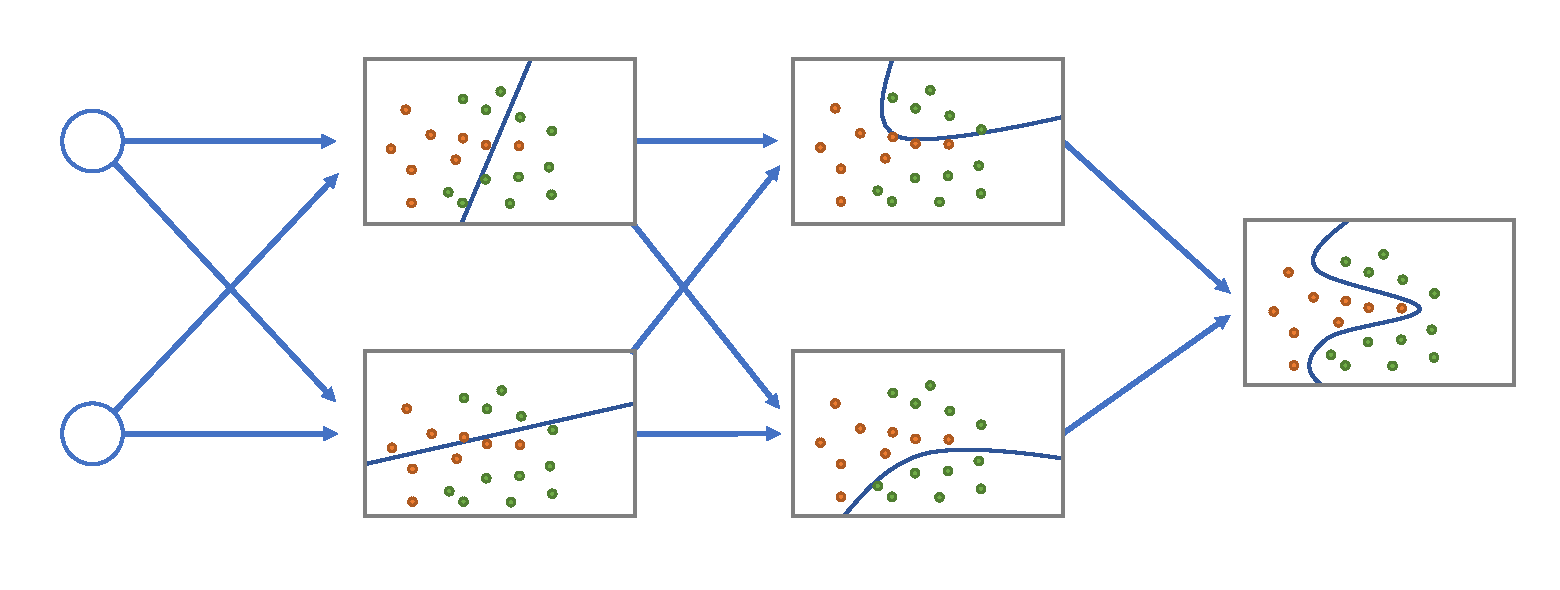
\includegraphics[width=\linewidth]{contents/chapter_3/resources/scheme_deep_understanding.pdf}
    \caption{Exemple simplifié d'une structure d’apprentissage profond. Ce modèle se compose de deux couches intermédiaires cachées~:~la première couche extrait des caractéristiques linéaires simples, tandis que la seconde couche par combinaison avec la première couche conduit à une extraction de caractéristiques plus complexes. Ainsi, la première couche s'apparente à un polynôme de degré 1, tandis que la seconde couche représente des fonctions de degré 2 et ainsi de suite.}
    \label{fig:scheme_deep_understanding}
\end{figure}

\subsection{Réseau neuronal convolutif}
\label{sec:convolutionnal_neural_network}
Les \gls{cnn} sont une extension des réseaux de neurones profonds, essentiellement utilisés dans un but de traitement de l'image. Moins développé par la littérature, ce principe de réseaux peut être étendu à des données telles que des signaux (1D) ou des volumes (3D).\par

Ces \gls{cnn} sont une réponse à l'application des \gls{ann} à des problématiques impliquant des données images et des contraintes multiples qu'ils comportent. Parmi ces contraintes de l'application des \gls{ann} aux images, peuvent être évoqués~:~
\begin{inlinerate}
    \item les \textbf{nombreuses connexions et paramètres requis},
    \item l'\textbf{absence d'utilisation de la cohérence de l'information spatiale},
    \item et la \textbf{dépendance} du réseau à la taille des informations d'entrée.
\end{inlinerate}\par

Ainsi, ces réseaux font appel à des couches de convolution permettant de résoudre ces trois principales contraintes. D'une part, la convolution permet de réduire fortement le nombre de paramètres d'entraînement, le réseau n'est ainsi plus entièrement \textit{connecté}. Certaines optimisations récentes consistent à remplacer les filtres de convolution 2D par une succession de filtres 1D horizontaux et verticaux, proposant des résultats semblables et réduisant fortement le nombre de paramètres. D'autres part, la convolution permet d'apporter une logique à la dimension spatiale des données ainsi qu'une indépendance à la taille. En effet, le réseau n'est plus entièrement connecté et donc ne dépend plus d'une taille fixe, et peut ainsi traiter des données de tailles différentes mais qui doivent respecter une taille minimum. Le traitement des données par ces couches de convolution porte le nom de carte d'activation, maximum quand le produit de convolution est en phase.\par

% \begin{equation} 
%     \label{eq:convolution_integral}
%     \begin{split}
%         (f\ast g) (x) = \int_{-\infty}^{+\infty} f(x-t)g(t) \, \mathrm dt = \int_{-\infty}^{+\infty} f(t)g(x-t) \, \mathrm dt
%     \end{split}
% \end{equation}

\clearpage

\subsection{Transfert de connaissances}
\label{sec:transfer_learning}
L’apprentissage par transfert est une technique connexe à l’apprentissage profond défini comme « faisant référence à la situation où ce qui a été appris dans un contexte \ldots est exploité pour améliorer la généralisation dans une autre contexte »~\cite{Ngiam2011}. Cette discipline s’inscrit dans le champ de \textbf{l’adaptation de domaine}, définie comme le transfert des connaissances d’un domaine $D_S$, défini par l’hypothèse $h: X_S \rightarrow Y_S$, vers un domaine cible $D_T$ afin de satisfaire $h: X_T \rightarrow Y_T$. Son champ d'application n'est pas limité aux réseaux d'apprentissage profond, mais les contraintes qui leurs sont associées font de ces techniques une ressource utile.\par

En effet, ces solutions permettent de réduire les difficultés liées à la grande quantité de ressources de calcul, de temps, mais également de données mobilisées nécessaires à un entraînement depuis sa base. Le modèle d’apprentissage attendu est alors initialement plus performant, croît plus efficacement et est plus performant qu’un apprentissage spécifique (\Cref{fig:learning_curves}).\par

Néanmoins, cette solution n’est envisageable que lorsque l’apprentissage, réalisé lors de la première tâche, généralise suffisamment le phénomène observé. Ainsi, il est d’usage courant de ne spécifier lors du transfert que la couche finale de classification du réseau, les premières couches étant employées comme extracteur général de caractéristiques. Toutefois, certaines méthodes de la littérature s’accordent sur l'entraînement conjoint des couches de classification ainsi que des couches de convolutions hautes, considérées comme moins génériques.\par

\begin{figure}[H]
    \centering
    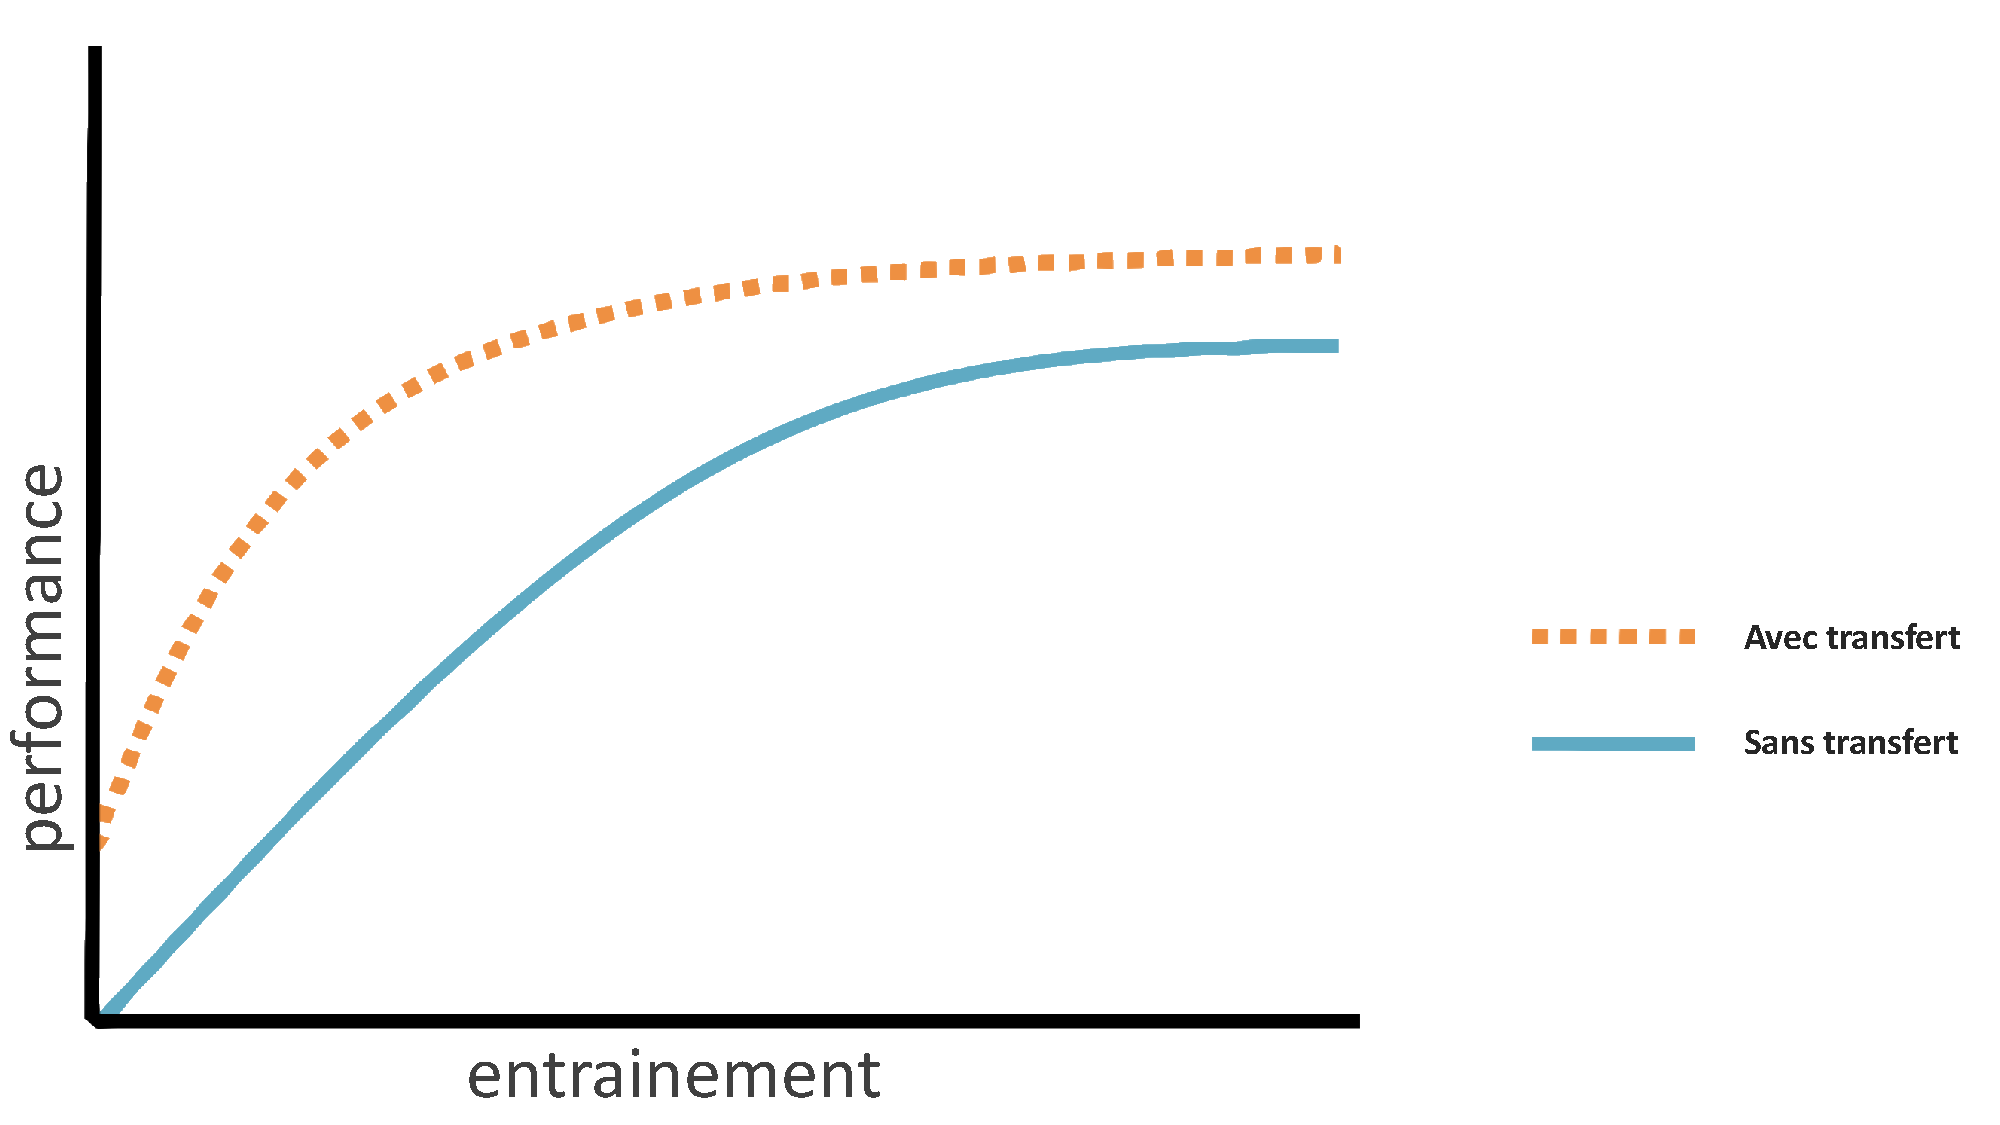
\includegraphics[width=\linewidth]{contents/chapter_3/resources/example_learning_curves.pdf}
    \caption{Exemple d'attentes liées à un apprentissage par transfert en opposition à un apprentissage classique.}
    \label{fig:learning_curves}
\end{figure}
\clearpage

\section{Paramétrage et évaluation de modèles prédictifs}
\label{sec:models_settings}
Cette partie se concentre sur l'évaluation de modèles de prédiction et présente la problématique de \textbf{biais}. Ses origines et ses risques associés sont présentés ainsi que les potentielles méthodes permettant de s'en affranchir.\par

\subsection{Généralisation de modèles}
\label{subsec:generalized_models}
À l'aide de couples d'entrée et de sortie mis à disposition, ces modèles sont capables d’apprendre une relation en la \textit{généralisant} et d’estimer de nouvelles sorties sur de nouvelles données. Il est pour cela nécessaire de parvenir à isoler l'information responsable de ce cheminement, plus ou moins séparable, en cause souvent la qualité de~:
\begin{inlinerate}
    \item l'hypothèse formulée, c’est-à-dire si la relation qui lie l'observation et sa conséquence est directe mais également vraie dans toute circonstance,
    \item l'information possédée, c’est-à-dire si l'information est juste pour répondre à la problématique cible (qualité de l'observation, rapport signal sur bruit, \ldots).
\end{inlinerate}\par 

Ce problème, évoqué dans la littérature porte le nom de « dilemme de biais et variance », dans lequel le biais représente le manque de relation pertinente entre données d’entrée et de sortie et où la variance représente l’influence du modèle au petites fluctuations souvent issues de bruit. Ces termes sont intrinsèquement liés aux problématiques respectives de \textbf{sous-apprentissage} et \textbf{sur-apprentissage}. La \Cref{fig:example_underfit_overfit} reprend de manière visuelle ces problématiques, et les exprime selon un jeu d’entraînement et de test. À noter que le sur-apprentissage peut être limité par l’utilisation de termes de régularisation, de schémas de validation de modèle adaptés ou l’utilisation d’ensembles de données suffisantes.\par
 
\begin{figure}[H]
    \centering
    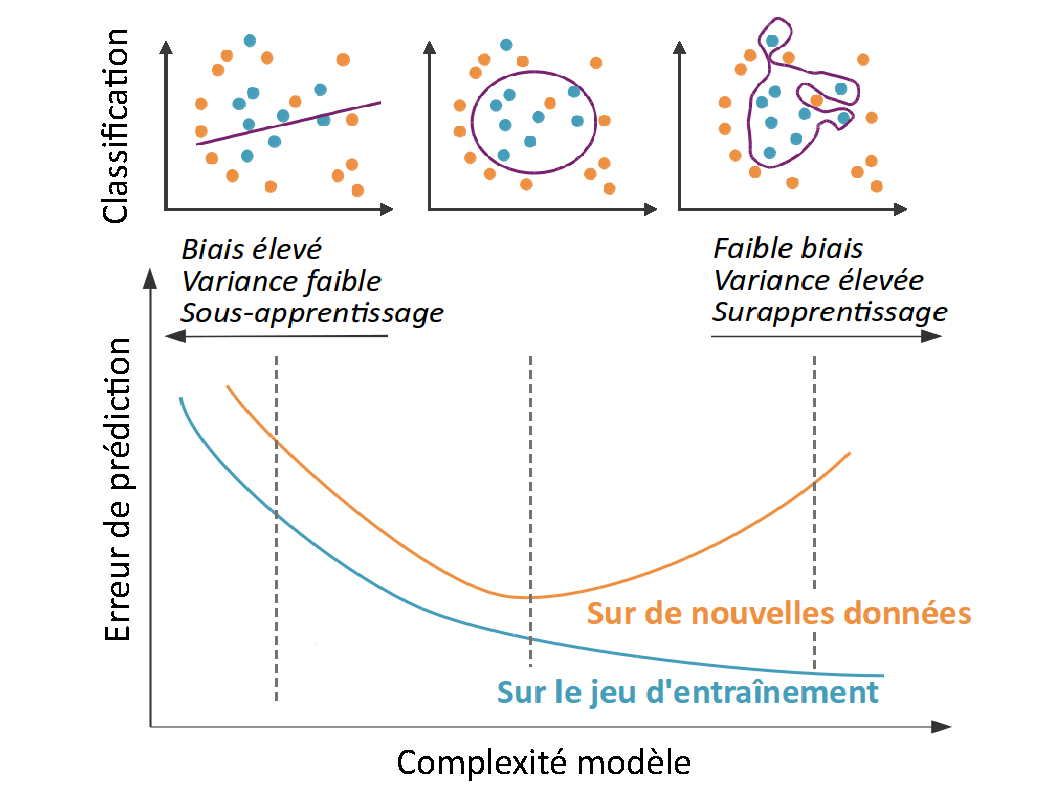
\includegraphics[width=0.85\linewidth]{contents/chapter_3/resources/example_underfit_overfit.pdf}
    \caption{Exemple de dilemme de biais et de variance. À gauche, un cas de sous-apprentissage, ce modèle est une sous approximation du phénomène observé. À droite, un cas de sur-apprentissage, le modèle ne généralise pas suffisamment le phénomène observé.}
    \label{fig:example_underfit_overfit}
\end{figure}

\subsection{Choix de métriques}
\label{subsec:metrics}
Le choix des métriques représente une part importante de la problématique de ce manuscrit pour la mise en place de modèles d’apprentissage. D'une part, ce choix permet d'orienter la sélection d'un modèle en particulier et d'autre part, permet de retenir les performances attendues par ce dernier sur des données extérieures au jeu de données employé.\par

L’un des principaux outils à disposition afin d'évaluer la performance est la matrice de confusion, schématisé sur la \Cref{fig:scheme_confusion_matrix}. Elle permet de faire correspondre les classes réelles et prédites~:~la diagonale de cette matrice fait figurer les prédictions correctement réalisées par le modèle, tandis que les éléments restants renseignent sur les prédictions erronées. Dans une situation à deux classes ou \textit{binaire}, cette matrice fait ainsi ressortir quatre mesures~:
\begin{itemize}
	\item les \textbf{vrais positifs}, les éléments de la classe positive détectés comme positif,
	\item les \textbf{vrais négatifs}, les éléments de la classe négative détectés comme négatif,
	\item les \textbf{faux positifs}, les éléments de la classe négative détectés comme positifs,
	\item les \textbf{faux négatifs}, les éléments de la classe positive détectés comme négatifs.
\end{itemize}\par

\begin{figure}[H]
    \centering
    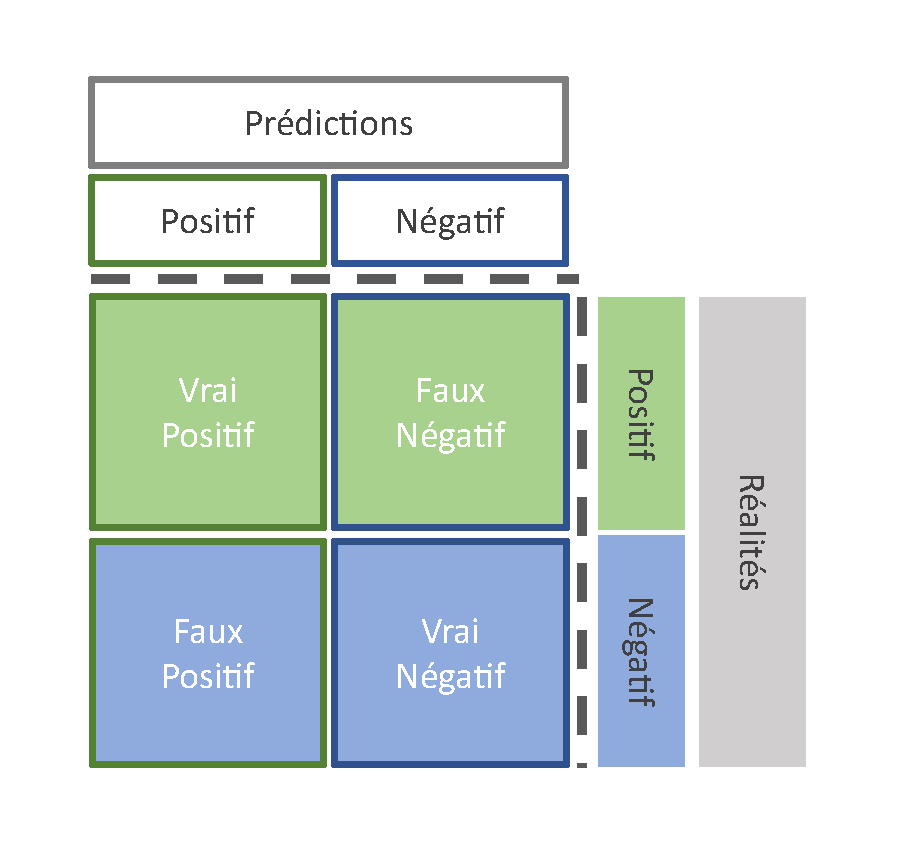
\includegraphics[width=\linewidth]{contents/chapter_3/resources/scheme_confusion_matrix.pdf}
    \caption{Schéma représentatif d’une matrice de confusion, qui met en avant une situation binaire.}
    \label{fig:scheme_confusion_matrix}
\end{figure}

Bien que déjà réduite, l'information de cette matrice est encore très riche et difficile à utiliser comme critère de sélection. Pour cela, diverses métriques éprouvées sont à envisager selon la problématique de recherche. Parmi les plus courantes d'entre elles, les critères de \textbf{précision}, \textbf{sensibilité} (également appelé \textbf{rappel}) ou encore \textbf{spécificité} sont pléthores dans la littérature mais ont tendance à ne capter qu'une partie du problème. Par exemple, la sensibilité est un critère très important en médecine ou détection de fraude, mais ne qualifie en rien la spécificité du modèle. De même, la moyenne fait également partie des critères extraits dans le domaine de l'intelligence artificielle, mais peut également manquer de sens en cas de non balancement de l'information~\cite{Guo2008} ou même ne pas mettre en avant un important gouffre entre spécificité et sensibilité. Ces métriques sont représentées de manière graphique sur la \Cref{fig:scheme_confusion_metrics} ou sous forme mathématique sur l'\Cref{eq:metrics_basics}.\par

\begin{figure}[H]
    \centering
    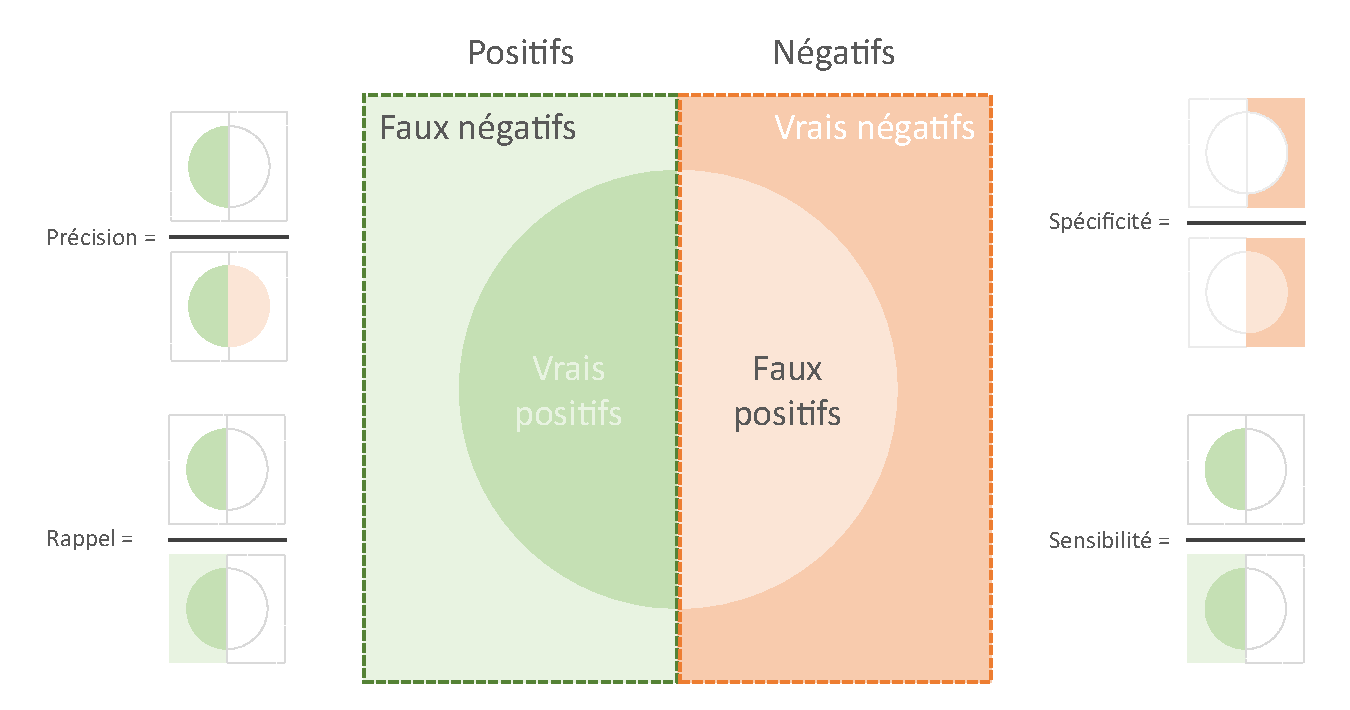
\includegraphics[width=\linewidth]{contents/chapter_3/resources/scheme_confusion_metrics.pdf}
    \caption{Schéma représentatif des principales métriques obtenues à partir de la matrice de confusion~:~la \textit{précision}, le \textit{rappel} ou la \textit{sensibilité} et la \textit{specificité}.}
    \label{fig:scheme_confusion_metrics}
\end{figure}

\begin{equation} 
    \label{eq:metrics_basics}
    \begin{split}
    Sensibilit\acute{e} &= VP/(VP+FN) \\
    Rappel &= Sensibilit\acute{e} \\	
    Sp\acute{e}cificit\acute{e} &=  VN/(VN+FP) \\
    Pr\acute{e}cision &= VP/(VP+FP) \\
    Moyenne &= (VP+VN)/(VP+VN+FP+FN)
    \end{split}
\end{equation}

Dans ce cas, il peut être préférable de privilégier des métriques plus robustes, dans le cadre de données non balancées. La plupart des méthodes s’accordent sur l’utilisation de métriques tels que le \fscore{}, associant conjointement sensibilité et précision, par principe de la moyenne harmonique~\cite{Guo2008}. L'\Cref{eq:metrics_fscore} met à disposition l'expression générique de cette métrique, dont le paramètre $\beta$ permet de moduler l'importance de la précision ou du rappel. L'influence de ce paramètre est neutre lorsque sa valeur est égale à 1 comme dans le cas du \fscore.\par
 
\begin{equation} 
    {F_\beta \: score}=(1+\beta^2)*(Pr\acute{e}cision*Rappel)/((\beta^2*Pr\acute{e}cision)+Rappel)
    \label{eq:metrics_fscore}
\end{equation}
 
Une autre métrique permettant de se prémunir de ces effets de non balancement de l'information et celui de l'\acs{auc} et découlant de la courbe \gls{roc} dont le principe est résumé sur le schéma \Cref{fig:scheme_roc_curve}). La courbe \gls{roc} est tracée à partir des informations de spécificité / sensibilité et par variation d'une valeur seuil appliquée au modèle de prédiction, tandis que l'\gls{auc} correspond à l'intégration de l'aire de cette courbe. Ainsi, l'\gls{auc} est robuste au non-balancement de données mais ses valeurs sont optimistes sur des modèles de prédiction dont la variation du seuil est homogène vis-à-vis des résultats.\par

\begin{figure}[H]
    \centering
    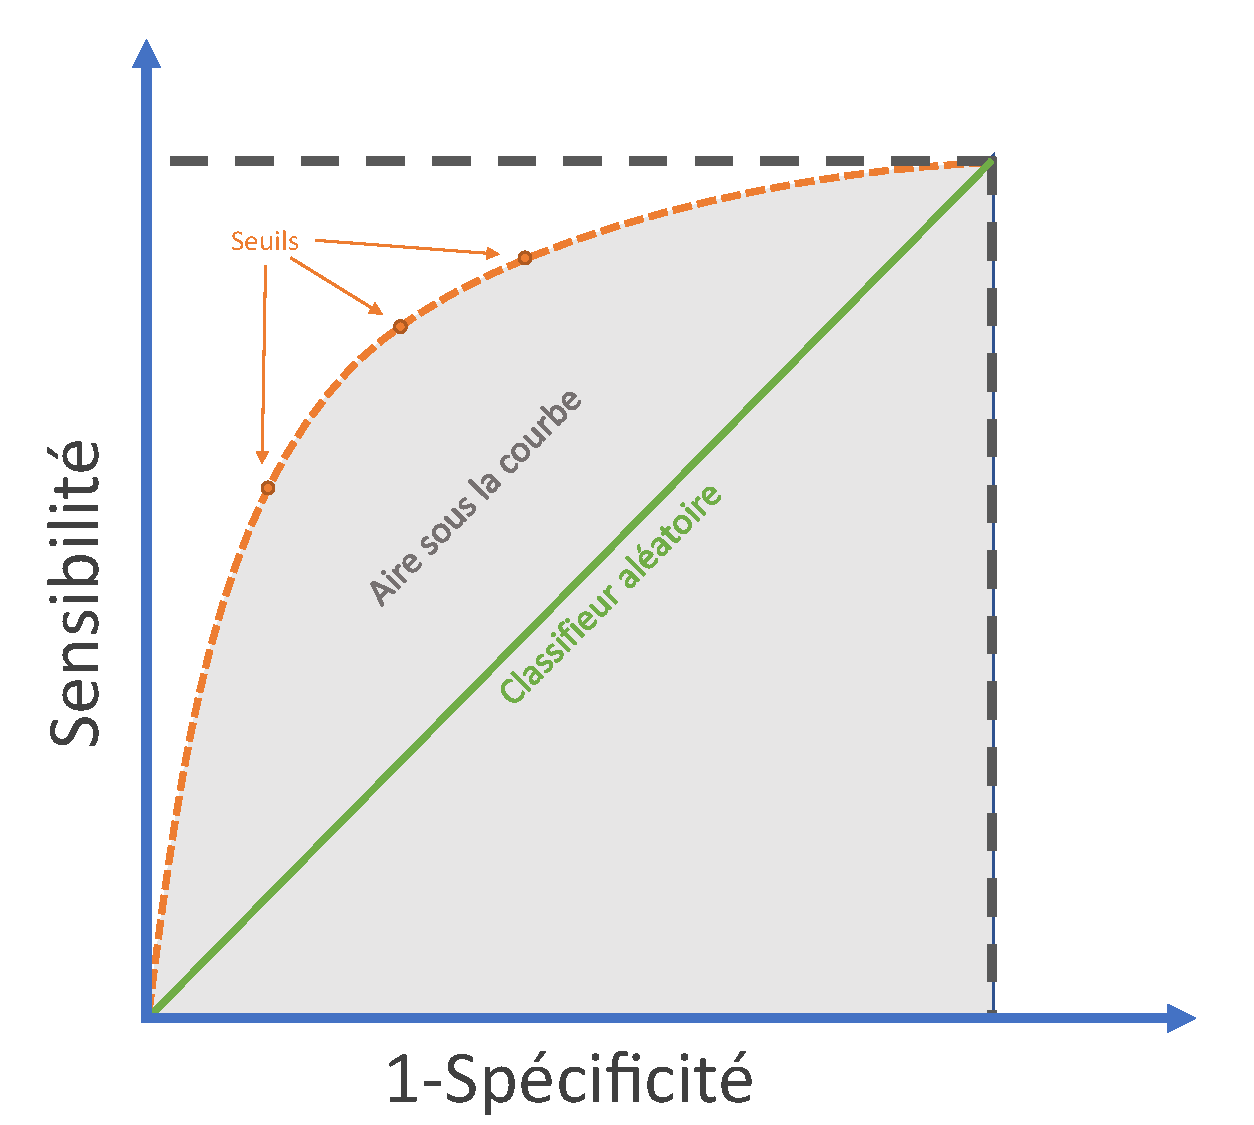
\includegraphics[width=0.80\linewidth]{contents/chapter_3/resources/scheme_roc_curve.pdf}
    \caption{Schéma de courbe \gls{roc} en orange et \gls{auc} en gris.}
    \label{fig:scheme_roc_curve}
\end{figure}

D'autres alternatives moins biaisées ont également été formulées~\cite{Sokolova2006}. Néanmoins le \fscore{} et l'\gls{auc} sont couramment utilisés dans des articles cliniques et constituent une des bases de ce travail.\par
\clearpage

\subsection{Réglages des hyperparamètres}
\label{subsec:hyperparameter}
Avant d’entrer plus en profondeur dans le sujet, il est nécessaire de revenir sur le terme \textbf{d’hyperparamètres}. Il caractérise les paramètres d'un processus d'apprentissage automatique dont le réglage doit être effectué avant la phase d'entraînement et dont les valeurs dépendent des données à traiter. Le réglage des hyperparamètres peut rarement être déterminé par la simple observation des données, et nécessite ainsi un réglage en fonction de chaque situation rencontrée.\par

L’une des premières techniques permettant ce réglage consiste à définir une \textit{grille} de ces hyperparamètres, contenant pour chacun, leurs possibles variations~\cite{Liu2006}. Il s'agit de la méthode la plus équitable puisqu'elle consiste à évaluer chaque combinaison par comparaison des performances finales (voir la \Cref{fig:example_hyperparameter_selection} - Gauche). Néanmoins, elle possède deux limitations majeures, dont~:
\begin{itemize}
    \item son \textbf{temps de calcul}, qui va croître de manière exponentielle en fonction du nombre d'hyperparamètres à valider,
    \item sa \textbf{précision}, qui va dépendre du pas choisi pour chacun des paramètres.
\end{itemize}\par

La seconde technique consiste à définir un \textit{espace} de recherche dont la distribution de chaque hyperparamètre sera choisie, ainsi qu'un nombre d'évaluations à réaliser pour déterminer la meilleure combinaison possible. Ce nombre d'évaluations est ensuite réalisé sous forme de tirage aléatoire, effectué à l'intérieur de cet espace de recherche défini~\cite{bergstra2012} (voir la \Cref{fig:example_hyperparameter_selection} - Droite). Cette méthode possède l'avantage d'être prévisible en termes de temps puisque le nombre de combinaisons évaluées est défini au préalable et quelles que soient les proportions de l'espace. Néanmoins, cette méthode possède également des inconvénients comme la représentation des tirages au sein de l'espace défini.

\begin{figure}[H]
    \centering
    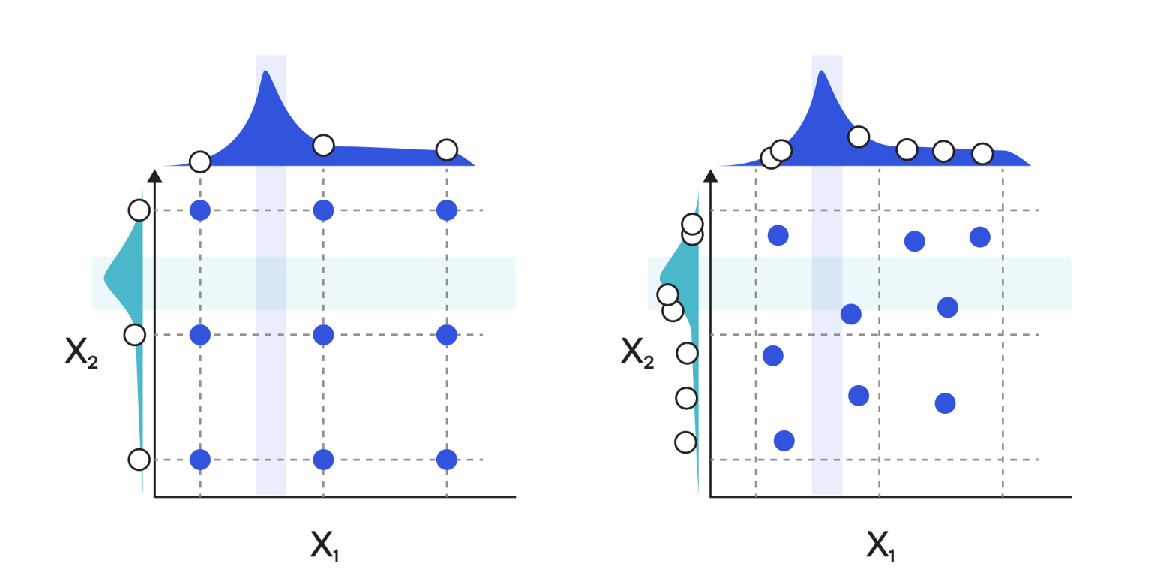
\includegraphics[width=\linewidth]{contents/chapter_3/resources/example_hyperparameter_selection.pdf}
    \caption{Exemple de recherche sur deux hyperparamètres $X_1$ et $X_2$. À gauche, une recherche sous forme de grille rigide, dans laquelle chaque combinaison est évaluée. À droite, une recherche aléatoire de ces hyperparamètres.}
    \label{fig:example_hyperparameter_selection}
\end{figure}

\subsection{Méthodes d'évaluation}
Divers aspects sont évoqués pour permettre l'ajustement des modèles dans la \Cref{subsec:hyperparameter} ainsi que la mesure de leurs performances dans la \Cref{subsec:metrics}. Il est nécessaire d'orchestrer cet ensemble afin d'obtenir la meilleure attente possible d'un modèle de prédiction, tout en conservant une mesure pertinente permettant de renseigner sur la fiabilité de ce modèle et de ses prédictions futures dans des situations où la vérité terrain n'est pas connue. En effet, l'évaluation d'un modèle de prédiction sur des données identiques à celles utilisées constitue un biais, par l'utilisation de connaissances \textit{a posteriori}. De même, l'ajustement des hyperparamètres rentre dans cette catégorie de l'entraînement, et l'évaluation ne peut se faire sur des données ayant servi à les déterminer. Par ailleurs, une telle évaluation permet de détecter les problèmes de sous-apprentissage et sur-apprentissage évoqués en \Cref{subsec:generalized_models}.\par

La méthode \textbf{holdout} est la plus simple d'entre elles et consiste à diviser l’échantillon de données en deux sous-ensembles respectivement d'entraînement et de test. Il est important lors de cette étape de vérifier que les données présentes dans chacun de ces sous-ensembles soient représentatives de chaque classe présente dans la problématique. Les données spécifiées pour le test restent ainsi non utilisées jusqu'à leur confrontation au modèle définitif qui est alors évalué sur ces dernières. Le principal inconvénient de cette méthode est que seule une partie du jeu de données sert d'évaluation à la méthode développée. Néanmoins, cette méthode est rapide à exécuter puisqu'elle ne nécessite l'entraînement que d'un modèle. Cette méthode est schématisée sur la \Cref{fig:scheme_holdout_cv} - Gauche.\par

La méthode de \textbf{validation croisée} permet d'étendre la méthode précédente à l'ensemble du jeu de données et d'obtenir un score moins biaisé. Pour cela, le jeu de données est subdivisé en \textbf{$k$ échantillons}, servant à tour de rôle de jeu de test, le reste de ces données étant réservé à l'entraînement. Ce principe de fonctionnement génère ainsi $k$ modèles de prédictions et autant de scores d'évaluation qui se résument à une unique valeur par application d'une fonction de moyenne. Le principal inconvénient de cette méthode est son temps de réalisation puisqu'elle nécessite l'entraînement d'autant de modèles que d'échantillons. Cette méthode est schématisée sur la \Cref{fig:scheme_holdout_cv} - Droite.\par

\begin{figure}[H]
    \centering
    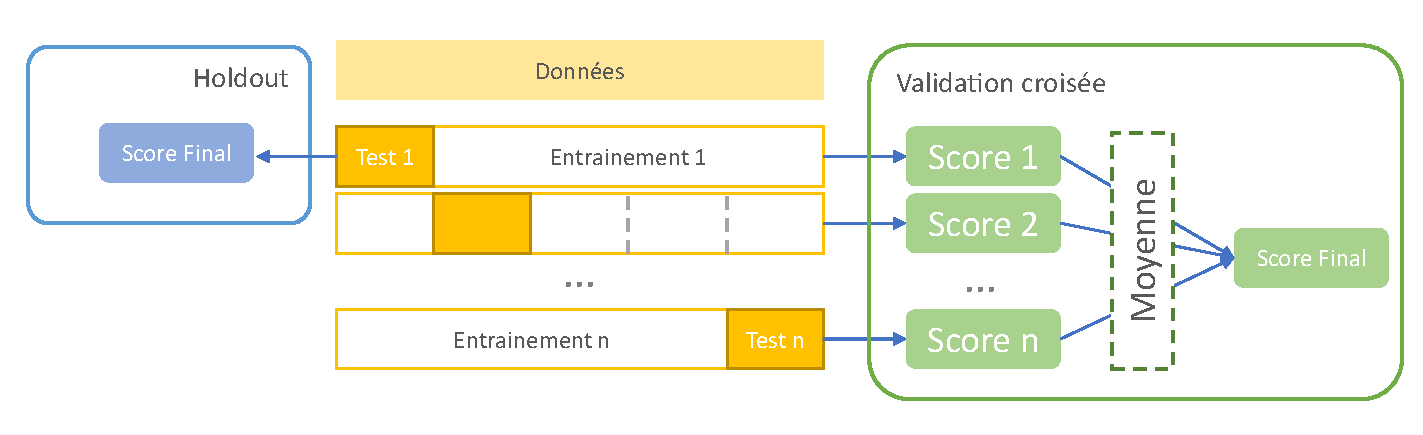
\includegraphics[width=\textwidth]{contents/chapter_3/resources/scheme_holdout_cv.pdf}
    \caption{Schéma des principes des deux approches majeures d'évaluation de modèles. À gauche, la méthode de \textit{holdout} ; À droite, la méthode de \textit{validation croisée}.}
    \label{fig:scheme_holdout_cv}
\end{figure}

Ce travail s'intéresse à la technique de validation croisée ainsi qu'à la valeur moyenne renvoyée par celle-ci. Afin de rendre cette information plus complète, la valeur de l'écart-type est conjointement calculée à partir des évaluations réalisées sur les divers échantillons, jugée fiable afin de mesurer la stabilité du processus vis-à-vis des données~\cite{Kim2009}. La plupart des travaux ayant recours à la validation croisée emploient une valeur $k$ comprise entre 5 et 10, jugée suffisante pour l'obtention de valeurs de moyenne et écart-type dans un temps de calcul raisonnable~\cite{James2013}. Néanmoins, il est possible d'amener ce principe à l'extrême en choisissant la plus petite valeur possible pour un lot dédié à l'évaluation soit la taille d'une donnée. Cette valeur $k$ devient égale au nombre de données à traiter, devenant un schéma qualifié de \textit{leave-one-out} ou littéralement \textit{en laisser un de côté}. Mais ce type de schéma de validation souffre généralement d'une variance élevée, surtout lorsque les données contiennent des valeurs aberrantes~\cite{Bengio2004}.\par

Ces deux méthodes répondent à la problématique de l'évaluation, mais n'apportent pas de solution quant au choix des hyperparamètres. En effet, utiliser un schéma de validation croisée pour régler et évaluer les modèles conduit inévitablement à surestimer les performances du modèle~\cite{Tsamardinos2014}. Ce type de démarche revient à ajuster au mieux une courbe à un nuage de points tout en affirmant que ces mêmes données correspondent à des données inconnues. L'une des solutions à ce problème est l'utilisation d'un double schéma de validation, dont l'un des plus fonctionnels actuellement est celui de la \textbf{validation croisée imbriquée}~\cite{Cawley2010}. Le principe de cette méthode est schématisé sur la \Cref{fig:scheme_hyperparameter_process}, laquelle se décompose en~:
\begin{itemize}
    \item une boucle \textbf{externe}, permettant d'évaluer un modèle à partir de données de \textbf{test},
    \item une boucle \textbf{interne}, permettant de valider un modèle et ses réglages à partir de données de \textbf{validation}.
\end{itemize}\par
  
\begin{figure}[H]
    \centering
    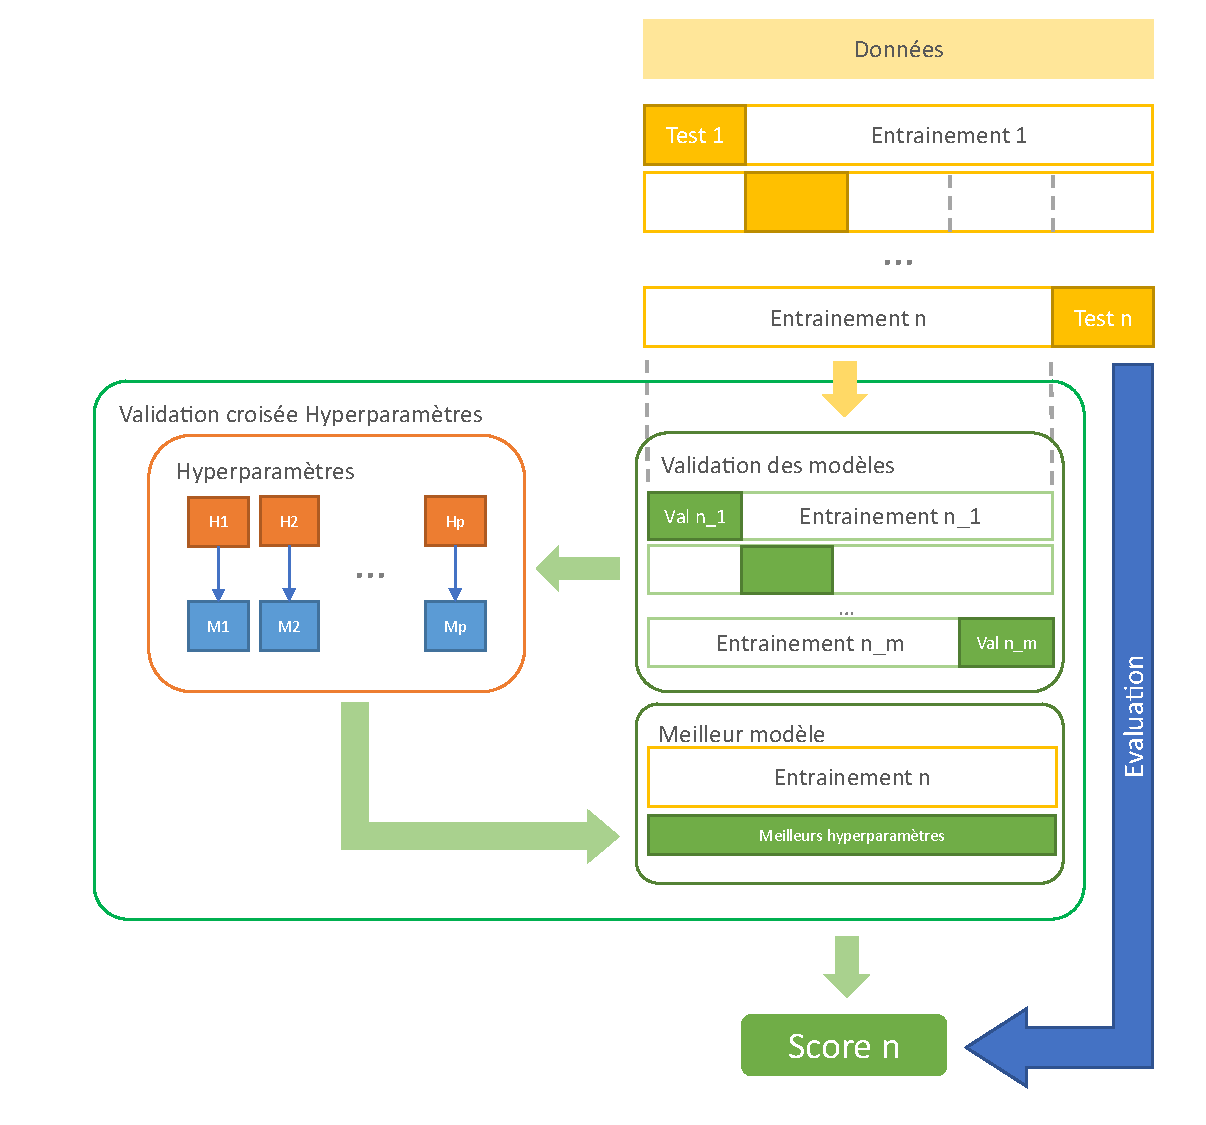
\includegraphics[width=0.9\linewidth]{contents/chapter_3/resources/scheme_hyperparameter_process.pdf}
    \caption{Schéma de la validation croisée imbriquée assurant le choix de la meilleure combinaison d'hyperparamètres et assurant une évaluation robuste des performances du modèle.}
    \label{fig:scheme_hyperparameter_process}
\end{figure}\par

\clearpage

\section{Fusion d’informations}
\label{sec:fusion_information}
Dernier aspect de ce sujet, la fusion d’informations se définit comme l’action de « combiner des informations issues de plusieurs sources afin d’améliorer la prise de décision »~\cite{Bloch2003}. Cette fusion se retrouve dans de nombreux domaines d'application dont celui de la santé ou encore de la biométrie, et peut être considérée comme un moyen d'augmenter la fiabilité de systèmes. L'intérêt croissant pour ce domaine correspond, entre autres, à une réponse de l'augmentation et de la diversification du nombre de capteurs présents. L'ouvrage de Bloch~\cite{Bloch2003} justifie la fusion d'informations, par différentes notions auxquelles chaque capteur est soumis, dont~:
\begin{itemize}
    \item \textbf{l'incertitude}~:~c’est-à-dire son « degré de conformité avec la réalité ».
    \item \textbf{l'imprécision}~:~définie comme une « mesure du défaut quantitatif de connaissance, sur une mesure ».
    \item \textbf{l'incomplétude}~:~correspond à « l'absence d'information d'une source sur des aspects du problème ».
\end{itemize}\par

Cette fusion est indispensable pour permettre la réalisation de certaines tâches, l'effet de McGurk est un exemple concret de la \textit{complémentarité} de la vision et de l'audition dans le rôle de la perception de la parole, mais également de la difficulté à gérer les \textit{conflits} d'informations sur ces deux sources séparées~\cite{Mcgurk1976}. L'ouvrage de Bloch~\cite{Bloch2003} définit trois termes propres à cette fusion~:
\begin{itemize}
    \item \textbf{le conflit}~:~l'une des notions pouvant conduire à une mauvaise interprétation du système lorsque plusieurs informations contradictoires sont reçues.
    \item \textbf{la redondance}~:~l'apport multiple d'une même information, pouvant dans l'idéal permettre de réduire les incertitudes et les imprécisions.
    \item \textbf{la complémentarité}~:~généralement des sources, liée à un apport de caractéristiques différentes permettant l'accès à une information globale et de lever des ambiguïtés.
\end{itemize}\par

Il est nécessaire également de caractériser le résultat de la fusion d'informations. Il est relativement difficile d'obtenir une vision commune sur les divers niveaux et termes associés. Ainsi, ce travail se réfère à l'une d'entre elles~\cite{Dasarathy1997} proche de cette problématique. Trois niveaux de fusion y sont décrits~:
\begin{itemize}
    \item le \textbf{niveau bas}, considéré comme étant la fusion sur les données,
    \item le \textbf{niveau moyen}, considéré comme la fusion des caractéristiques ou données plus abstraites,
    \item le \textbf{niveau haut}, considéré comme la fusion des décisions.
\end{itemize} Niveaux au sein desquels le processus de fusion d'informations peut aboutir à~:
\begin{inlinerate}
    \item une sélection,
    \item une transformation,
    \item une extraction,
    \item ou encore une classification de l'information.
\end{inlinerate} La \Cref{fig:scheme_overview_fusion} propose une schématisation macroscopique de ce concept.\par
 
\begin{figure}[H]
    \centering
    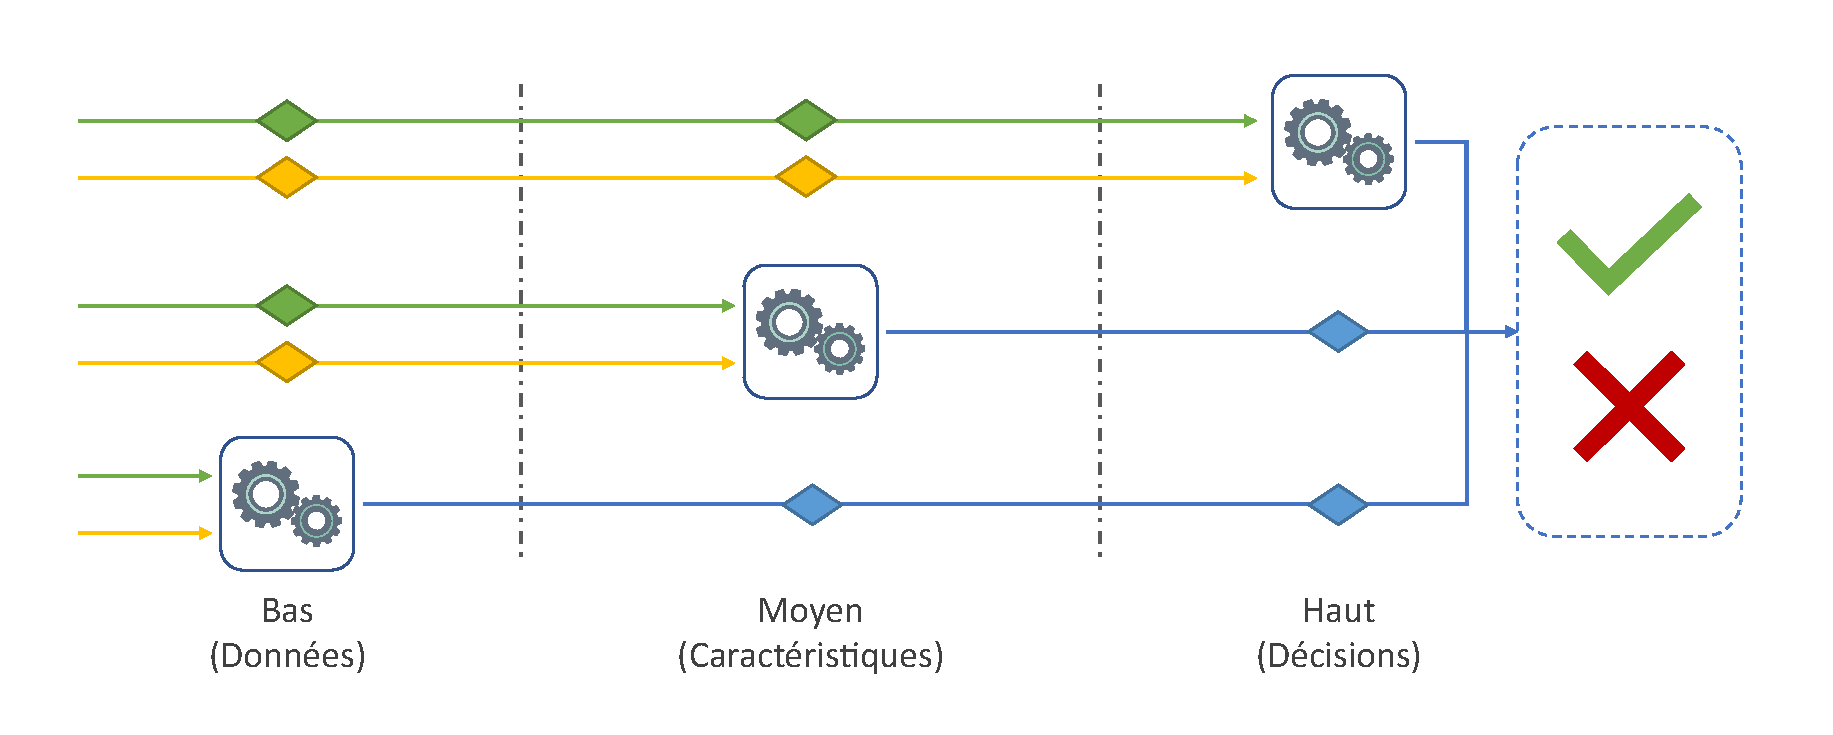
\includegraphics[width=\linewidth]{contents/chapter_3/resources/scheme_overview_fusion.pdf}
    \caption{Schéma des différents niveaux théoriques de fusion sur un schéma multimodal à deux capteurs. Le niveau bas représente le niveau le plus proche des données et des capteurs, le niveau moyen représente le niveau au plus proche de l'extraction de caractéristiques avancées, enfin le niveau haut représente le niveau de prise de décision.}
    \label{fig:scheme_overview_fusion}
\end{figure}\par

La fusion à \textbf{bas niveau} s'exerce au niveau du capteur, quand celui-ci bénéficie de plusieurs relevés d'informations physiques, ou après l'acquisition de données provenant de plusieurs capteurs. Cela va nécessiter une cohérence entre ces modalités~:~un référentiel, un repère commun permettant la mise en parallèle de ces dernières. La fusion à ce niveau consiste essentiellement à fournir une cohérence de ces modalités d'information, voire à réduire cette dernière afin de n'obtenir que celle jugée pertinente dans le cadre de son utilisation.\par

La fusion à \textbf{moyen niveau} s'exerce au niveau de caractéristiques, c’est-à-dire après un premier traitement de chacune des modalités pour n'extraire que les éléments nécessaires à la réalisation du processus. Il s'agit d'une mise en commun des vecteurs d'information dans leur totalité ou réduite, nécessitant dans ce second cas une sélection de l'information pertinente.\par

Enfin, la fusion à \textbf{haut niveau} s'exerce après les mécanismes de prise de décision. C’est-à-dire que les branches correspondant à chaque modalité exercent indépendamment leur prise de décision. Il est donc nécessaire de définir une stratégie permettant de privilégier une décision ou d'extraire une décision à partir de l'information. Deux catégories sont ainsi identifiables~:
\begin{inlinerate}
    \item la \textbf{sélection dynamique de modèle} de prédiction dans lequel l'objectif est de définir le modèle pertinent,
    \item et la \textbf{fusion de modèles} de prédiction dans lequel le but est d'obtenir une décision globale tenant compte des différentes décisions.
\end{inlinerate}\par

Plus particulièrement, dans le cadre de problématique binaire, la fusion de modèle comporte deux niveaux conceptuels de décision basés sur le type d'information mise à disposition par ces modèles. D'une part, le plus haut niveau reprend l'idée d'une fusion appliquée au \textbf{niveau décisionnel}. Seules les décisions issues de chaque modèle sont alors considérées selon diverses stratégies~:~le vote à la majorité ou encore la pondération des votes en sont deux représentants. D'autre part, le plus bas niveau reprend l'idée d'une fusion appliquée aux scores~\cite{Kittler1998}. Dans le cadre de problématiques à plusieurs classes, il est possible d'évoquer une troisième prise de décision au niveau du rang, c’est-à-dire en considérant la position de chaque classe prédite issue des divers modèles.\par


% \subsection{Équilibrage de données}
% Nous regroupons au travers de ce terme l’ensemble des problématiques relatives à notre jeu de données et à la représentation de ses classes. Dans le cas de pathologie de la peau, cela peut se caractériser par un jeu de données composé de 100 éléments dont 20~\% d’entre elles se réfèrent à des patients atteints de mélanomes et le reste à des patients sains. Nous constatons dans ce cas un déséquilibre entre les classes de ce jeu de données, qu’il nous faudra prendre en compte. Un tel jeu de données peut être qualifié de « non balancés », la répartition de ses classes n’étant pas égale en proportions.
% En effet, certains algorithmes de prédictions peuvent être biaisés, comme par exemple « l’algorithme des plus proches voisins » qui se composera de zones de forte densité privilégiant les données présentes en masse (exemple Figure 37). Un autre biais est également présent lors de l’extraction de métriques pour juger de la pertinence d’un modèle. En effet, dans le cas d’un classifieur qui prédirait constamment « sain », nous obtiendrons un score de 80~\% de précision sur notre jeu de données précédent.
  
% \begin{figure}[H]
%     \centering
%     \includegraphics[width=\linewidth]{contents/chapter_3/resources/unbalanced.pdf}
%     \caption{Illustration du problème de données non balancées sur l’algorithme KNN. La densité des données bleu étant supérieure, des prédictions à la frontière de nos deux classes favorisent la classe bleue.}
%     \label{fig:unbalanced}
% \end{figure}

% Plusieurs méthodes existent dans la littérature, pour permettre de rétablir l’équilibre entre les différentes classes. Nous pouvons citer les deux principaux~:
% 	Le sur-échantillonnage, c’est-à-dire que nous gonflons les classes sous représentatives de manière à égaliser la population de la classe majoritaire (en créant de nouveaux éléments artificiels par exemple).
% 	Le sous-échantillonnage, c’est-à-dire que nous réduisons la population de l’ensemble des classes à celle de la classe minoritaire.
 
% \begin{figure}[H]
%     \centering
%     \includegraphics[width=\linewidth]{contents/chapter_3/resources/example_balancement_strategies.pdf}
%     \caption{Représentation de deux principales catégories de stratégie de balancement des données. Le suréchantillonnage tente d’augmenter la taille du jeu de données faible tandis que le sous échantillonnage tend à réduire la classe majoritaire. }
%     \label{fig:example_balancement_strategies}
% \end{figure}